%!TEX program = xelatex

\documentclass[compress]{beamer}
%--------------------------------------------------------------------------
% Common packages
%--------------------------------------------------------------------------
\definecolor{links}{HTML}{663000}
\hypersetup{colorlinks,linkcolor=,urlcolor=links}

\usepackage[english]{babel}
\usepackage{pgfpages} % required for notes on second screen
\usepackage{graphicx}

\usepackage{multicol}

\usepackage{tabularx,ragged2e}
\usepackage{booktabs}
\usepackage{multirow}

\setlength{\emergencystretch}{3em}  % prevent overfull lines

\usetheme{hri}
%% Display the navigation bullet even without subsections
%\usepackage{remreset}% tiny package containing just the \@removefromreset command
%\makeatletter
%\@removefromreset{subsection}{section}
%\makeatother
%\setcounter{subsection}{1}

%% Neat trick to have only one navigation bullet per subsection
%% http://tex.stackexchange.com/questions/64333/one-navigation-bullet-per-subsection-with-subsection-false-in-custom-beamer-them
\usepackage{etoolbox}
\makeatletter
\patchcmd{\slideentry}{\advance\beamer@xpos by1\relax}{}{}{}
\def\beamer@subsectionentry#1#2#3#4#5{\advance\beamer@xpos by1\relax}%
\makeatother

%% Neat trick to have only display the navigation bullets for the current subsection
%% http://tex.stackexchange.com/questions/23151/beamer-infolines-outer-theme-with-miniframe-bullets-only-for-the-current-section/45152#45152
%\setbeamertemplate{mini frame in other section}{}
%\usepackage{etoolbox}
%\makeatletter
%\let\beamer@section@set@min@width=\relax
%\patchcmd{\insertnavigation}{\hskip-1.875ex plus-1fill}{}{}{}
%\patchcmd{\sectionentry}{\hskip1.875ex plus 1fill}{}{}{}
%\patchcmd{\sectionentry}{\hyperlink{Navigation#3}{{\usebeamertemplate{section in head/foot shaded}}}}{}{}{}
%\patchcmd{\slideentry}{\usebeamertemplate{mini frame in other subsection}}{\usebeamertemplate{mini frame in other subsection of current section}}{}{}
%\patchcmd{\slideentry}{\usebeamertemplate{mini frame in other subsection}}{\usebeamertemplate{mini frame in other section}}{}{}
%\patchcmd{\slideentry}{\usebeamertemplate{mini frame in other subsection of current section}}{\usebeamertemplate{mini frame in other subsection}}{}{}
%\makeatother

\newcommand{\source}[2]{{\tiny\it Source: \href{#1}{#2}}}

\usepackage{tikz}
\usetikzlibrary{mindmap,backgrounds,positioning,patterns,calc}

\usepackage{pgfplots}
\pgfplotsset{compat=newest}

\graphicspath{{figs-lowres/}{figs/}}

\title{ROCO318 \newline Mobile and Humanoid Robots}
\subtitle{Part 2 -- Sensors and Perception}
\date{}
\author{Séverin Lemaignan}
\institute{Centre for Neural Systems and Robotics\\{\bf Plymouth University}}

\begin{document}

\licenseframe{github.com/severin-lemaignan/module-mobile-and-humanoid-robots}

\maketitle

\begin{frame}{Part 2 -- Sensors and perception}

    For further reading see Part C from (Siciliano and Khatib, 2008) or
    chapter 4 of (Siegwart and Nourbakhsh, 2004).

\end{frame}

\section{Sensor classification}\label{sensor-classification}

\begin{frame}{Sensor classification}

    \footnotesize
    \textbf{Proprioceptive} sensors

    \begin{itemize}

        \item
              measure values internally to the system (robot),
        \item
              \eg motor speed, wheel load, heading of the robot, battery status
    \end{itemize}

    \textbf{Exteroceptive} sensors

    \begin{itemize}

        \item
              information from the robots environment
        \item
              distances to objects, intensity of the ambient light, unique features.
    \end{itemize}

    \textbf{Passive} sensors

    \begin{itemize}

        \item
              energy coming from the environment
    \end{itemize}

    \textbf{Active} sensors

    \begin{itemize}

        \item
              emit their proper energy and measure the reaction
        \item
              better performance, but some influence on envrionment
    \end{itemize}

\end{frame}

\begin{frame}{Examples of classification (1/2)}

    \scriptsize

    \begin{tabular}{@{}p{4cm}p{4cm}ll@{}}
        \toprule
        {\bf General classification}\newline(typical use)                                                                             & \bf Sensor\newline Sensor system & PC or EC & A or P \\ \midrule
        \multirow{3}{\linewidth}{{\it Tactile sensors} \newline \tiny detection of physical contact or closeness; security switches}  & Contact switches, bumpers        & EC       & P      \\
                                                                                                                                      & Optical barriers                 & EC       & A      \\
                                                                                                                                      & Noncontact proximity sensors     & EC       & A      \\ \midrule
        \multirow{7}{\linewidth}{{\it Wheel/motor sensors} \newline \tiny wheel/motor speed and position}                             & Brush encoders                   & PC       & P      \\
                                                                                                                                      & Potentiometers                   & PC       & P      \\
                                                                                                                                      & Synchros, resolvers              & PC       & A      \\
                                                                                                                                      & Optical encoders                 & PC       & A      \\
                                                                                                                                      & Magnetic encoders                &          & A      \\
                                                                                                                                      & Inductive encoders               & PC       & A      \\
                                                                                                                                      & Capacitive encoders              & PC       & A      \\ \midrule
        \multirow{3}{\linewidth}{{\it Heading sensors}\newline \tiny orientation of the robot in relation to a fixed reference frame} & Compass                          & EC       & P      \\
                                                                                                                                      & Gyroscopes                       & PC       & P      \\
                                                                                                                                      & Inclinometers                    & EC       & A/P    \\ \bottomrule
    \end{tabular}

    PC: proprioceptive; EC: exteroceptive; A: active; P: passive; A/P: active/passive
\end{frame}

\begin{frame}{Examples of classification (2/2)}

    \scriptsize

    \begin{tabular}{@{}p{4cm}p{4cm}ll@{}}
        \toprule
        {\bf General classification}\newline(typical use)                                                                                         & \bf Sensor\newline Sensor system & PC or EC & A or P \\ \midrule
        \multirow{4}{\linewidth}{{\it Ground-based beacons}\newline\tiny localization in a fixed reference frame}                                 & GPS                              & EC       & A      \\
                                                                                                                                                  & Active optical of RF beacons     & EC       & A      \\
                                                                                                                                                  & Active ultrasonic beacons        & EC       & A      \\
                                                                                                                                                  & Reflective beacons               & EC       & A      \\ \midrule


        \multirow{5}{\linewidth}{{\it Active ranging}\newline\tiny reflectivity, time-of-flight, geometric triangulation}                         & Reflectivity sensors             & EC       & A      \\
                                                                                                                                                  & Ultrasonic sensor                & EC       & A      \\
                                                                                                                                                  & Laser range finder               & EC       & A      \\
                                                                                                                                                  & Optical triangulation (1D)       & EC       & A      \\
                                                                                                                                                  & Structured light (2D)            & EC       & A      \\ \midrule
        \multirow{2}{\linewidth}{{\it Motion/speed sensors}\newline\tiny speed relative to fixed or moving objects}                               & Doppler radar                    & EC       & A      \\
                                                                                                                                                  & Doppler sound                    & EC       & A      \\ \midrule
        \multirow{3}{\linewidth}{{\it Vision-based sensors}\newline \tiny visual ranging, whole image analysis, segmentation, object recognition} & CCD/CMOS camera(s)               & EC       & P      \\
                                                                                                                                                  & Visual ranging packages          &          &        \\
                                                                                                                                                  & Object tracking packages         &          &        \\ \bottomrule
    \end{tabular}


\end{frame}

%%%%%%%%%%%%%%%%%%%%%%%%%%%%%%%%%%%%%%%%%%%%%%%%%%%%%%%%%%%%%%%%%%%%%%%%%%%%%%%%%
%%%%%%%%%%%%%%%%%%%%%%%%%%%%%%%%%%%%%%%%%%%%%%%%%%%%%%%%%%%%%%%%%%%%%%%%%%%%%%%%%
\section[Characterizing Performance]{Characterizing Sensor Performance}\label{characterizing-sensor-performance}

\begin{frame}{Basic sensor response ratings (1/2)}

    \begin{itemize}
        \item {\bf Dynamic range}: ratio between lower and upper limits, sometimes expressed
              in decibels (dB, power)
              \[
                  \bubblemark{decibel}10\cdot \log_{10}\frac{P_{upper}}{P_{lower}}
              \]

              \bubble<1>[30]{decibel}{Multiplied by 10 to make the number a bit larger. That's why it's called
                  \emph{deci}Bel.}

              \begin{itemize}

                  \item<2->
                  \eg current measurement from 1 milliamp to 30 amps
                  \[
                      \bubblemark{twenty}20\cdot\log_{10}\frac{I_{upper}}{I_{lower}}=20\cdot\log_{10}\frac{30A}{0.001A}=90dB
                  \]
                  \bubble<2>[30][0.7cm]{twenty}{20 instead of 10 because square of current or voltage is proportional to power.}

                  \item<3->
                  \eg voltage measurement from 1 millivolt to 20 volts
                  \[
                      20\cdot\log_{10}\frac{I_{upper}}{I_{lower}}=20\cdot\log_{10}\frac{20V}{0.001V}=86dB
                  \]
              \end{itemize}

              \item<4-> {\bf Range}
              \begin{itemize}
                  \item upper and lower limits
              \end{itemize}



    \end{itemize}

\end{frame}

%%%%%%%%%%%%%%%%%%%%%%%%%%%%%%%%%%%%%%%%%%%%%%%%%%%%%%%%%%%%%%

\begin{frame}{Basic sensor response ratings (2/2)}

    \begin{itemize}
        \item {\bf Resolution}
              \begin{itemize}
                  \item minimum difference between two values
                  \item usually: lower limit of dynamic range = resolution
                  \item for digital sensors it is usually the A/D resolution,\\ \eg $ 5V / 255 $ (8 bit)

              \end{itemize}

        \item {\bf Linearity}

              \begin{itemize}
                  \item
                        variation of output signal as function of the input signal
                  \item
                        linearity is less important when signal is after treated with a
                        computer
              \end{itemize}

        \item {\bf Bandwidth or Frequency}

              \begin{itemize}
                  \item the speed with which a sensor can provide a stream of readings
                  \item usually there is an upper limit depending on the sensor and the
                        sampling rate
                  \item Lower limit is also possible, \eg acceleration sensor
              \end{itemize}

    \end{itemize}
\end{frame}

\begin{frame}{\emph{In Situ} Sensor Performance}

    Characteristics that are especially relevant for real
    world environments

    \begin{itemize}
        \item {\bf Sensitivity}

              \begin{itemize}

                  \item
                        ratio of output change to input change
                  \item
                        in real world environments, the sensor often has a high sensitivity to
                        other environmental changes, \eg illumination
              \end{itemize}

        \item {\bf Cross-sensitivity}

              \begin{itemize}

                  \item
                        sensitivity to environmental parameters that are orthogonal to the
                        target parameters
              \end{itemize}

        \item {\bf Error / Accuracy}

              \begin{itemize}

                  \item
                        difference between the sensor's output and the true value
              \end{itemize}
              \[
                  accuracy =  1 - \frac{|m-v|\bubblemark{error}}{v}
              \]
              $m$: measured value; $v$: true value
              \bubble<1>[160]{error}{= error}
    \end{itemize}
\end{frame}

\begin{frame}{\emph{In Situ} Sensor Performance}


    Systematic error \Rightarrow \textbf{deterministic} errors

    \begin{itemize}
        \item
              caused by factors that can (in theory) be modeled \rightarrow
              prediction
        \item
              \eg calibration of a laser sensor or of the distortion caused by the
              optics of a camera
    \end{itemize}

    Random error \Rightarrow \textbf{non-deterministic}

    \begin{itemize}

        \item
              no prediction possible
        \item
              however, they can be described probabilistically
        \item
              \eg hue instability of camera, black level noise of camera\ldots
    \end{itemize}

\end{frame}

\begin{frame}{Sampling rate}

    \textbf{Nyquist theorem}

    \begin{itemize}

        \item The sampling rate has to be at least \textbf{twice as high} as the
              fastest changes. If not, you are going to miss relevant information.
              \begin{center}
                  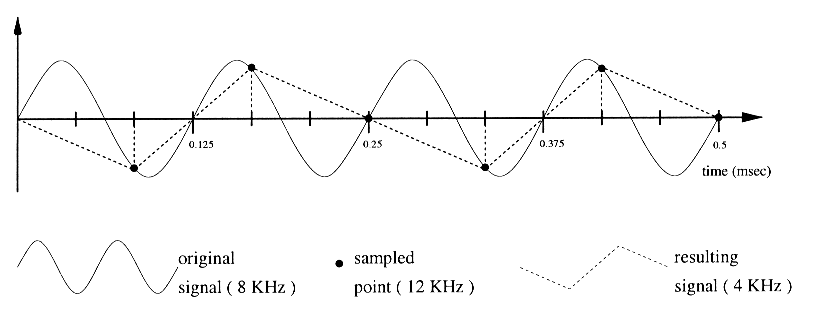
\includegraphics[width=0.8\linewidth]{nyquist}
              \end{center}

        \item \eg if sound signal changes at 3kHz, you have to sample at at least
              6kHz to not miss anything of the signal.
    \end{itemize}

\end{frame}

\begin{frame}{Nyquist: example}

    \begin{center}

        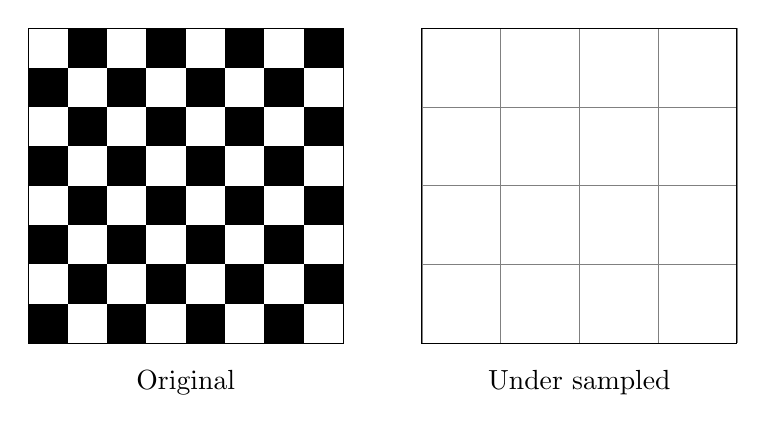
\begin{tikzpicture}[rectangle/.style={fill=black}]

            \node at (-2,-0.5) [anchor=center] {Original};
            \node at (3,-0.5) [anchor=center] {Under sampled};
            \foreach \x in {-4,...,-1} {
                \foreach \y in {0,...,3} {
                    \fill (\x,\y) rectangle (\x+0.5,\y+0.5);
                    \fill (\x+0.5,\y+0.5) rectangle (\x+1,\y+1);
                }
            }
            \draw[help lines] (1,0) grid (5,4);
            \draw (-4,0) rectangle (0,4);
            \draw (1,0) rectangle (5,4);

        \end{tikzpicture}
    \end{center}
    Under sampling results in \emph{aliasing} (in computer imaging this is
    tackled by anti-aliasing).

\end{frame}

\begin{frame}{Characterizing Error in Mobile Robotics}
    \begin{itemize}
        \item Mobile Robot has to perceive, analyze and interpret the state of the
              surrounding

        \item Measurements in real world environment are dynamically changing and
              error prone.

        \item Examples:

              \begin{itemize}
                  \item  changing illuminations

                  \item specular reflections

                  \item light or sound absorbing surfaces

                  \item cross-sensitivity of robot sensor to robot pose and robot-environment
                        dynamics

                        \begin{itemize}

                            \item
                                  rarely possible to model \rightarrow appear as random errors
                            \item
                                  systematic errors and random errors might be well defined in
                                  controlled environment.\\\emph{This is not the case for mobile robots
                                  !!}
                        \end{itemize}

              \end{itemize}
    \end{itemize}
\end{frame}

\begin{frame}{Multi-Modal Error Distributions: The Challenges in \ldots{}}

    Behavior of sensors modeled by probability distribution (random errors)

    \begin{itemize}
        \item usually very little knowledge about the causes of random errors

        \item often probability distribution is assumed to be symmetric or even
              Gaussian

        \item however, it is important to realize how wrong this can be!

        \item Examples:
              \begin{itemize}
                  \item Sonar (ultrasonic) sensor might overestimate the distance in real
                        environment and is therefore not symmetric.
                        \footnotesize Thus the sonar sensor might be best modeled by two
                        modes:

                        \begin{itemize}

                            \item mode for
                                  the case that the signal returns directly
                            \item mode for the case that the
                                  signals returns after multi-path reflections.
                        \end{itemize}

                  \item Stereo vision system might correlate to images incorrectly, thus causing
                        results that make no sense at all.
              \end{itemize}

    \end{itemize}
\end{frame}

%%%%%%%%%%%%%%%%%%%%%%%%%%%%%%%%%%%%%%%%%%%%%%%%%%%%%%%%%%%%%%%%%%%%%%%%%%
%%%%%%%%%%%%%%%%%%%%%%%%%%%%%%%%%%%%%%%%%%%%%%%%%%%%%%%%%%%%%%%%%%%%%%%%%
\section[Sensors Overview]{Overview of sensors often used on mobile robots}
\tableofcontents[currentsection]
%%%%%%%%%%%%%%%%%%%%%%%%%%%%%%%%%%%%%%%%%%%%%%%%%%%%%%%%%%%%%%%%%%%%%%%%%%%%%%%%%%%%%%%%%%
\subsection{Encoders}
\begin{frame}{Wheel / Motor Encoders}

    \footnotesize
    \begin{itemize}
        \item Measures position or speed of the wheels or steering.

        \item Wheel movements can be \textbf{integrated} to get an estimate of the robots
            position \rightarrow \textbf{odometry}

        \item Optical encoders are proprioceptive sensors
              \begin{itemize}
                  \item \footnotesize Due to errors (slippage etc.) the position estimate in relation to a
                        fixed reference frame is only valuable for short movements
              \end{itemize}

        \item Typical resolutions: 2000 increments per revolution
              \begin{itemize}
                  \item \footnotesize For high resolution: interpolation
              \end{itemize}

        \item Quadrature encoder (two emittor/detector pairs)
              \begin{itemize}
                  \item \footnotesize Gives direction and 4 times higher resolution.
              \end{itemize}
    \end{itemize}

    \begin{center}
        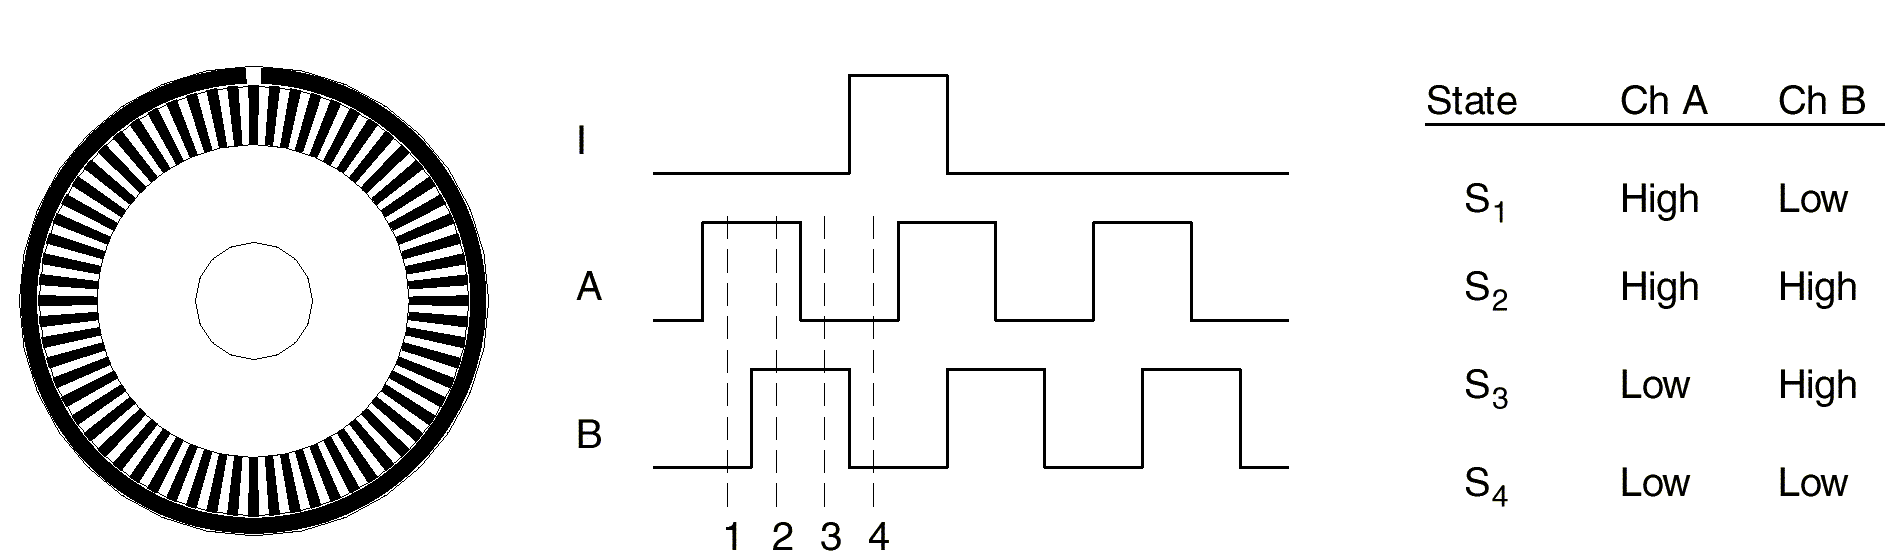
\includegraphics[width=0.9\linewidth]{encoders1}
    \end{center}

\end{frame}

\begin{frame}{Wheel / Motor Encoders}
    \centering

    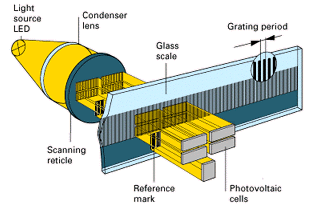
\includegraphics[width=0.45\columnwidth]{encoders2}
    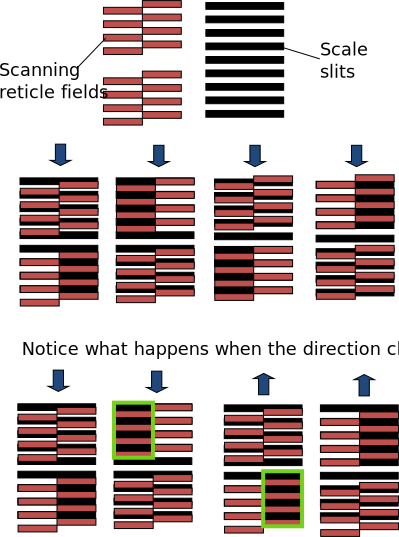
\includegraphics[width=0.45\columnwidth]{encoders}



\end{frame}

\begin{frame}{Wheel / motor encoders}


    \begin{columns}
        \begin{column}{0.5\linewidth}
            \centering

            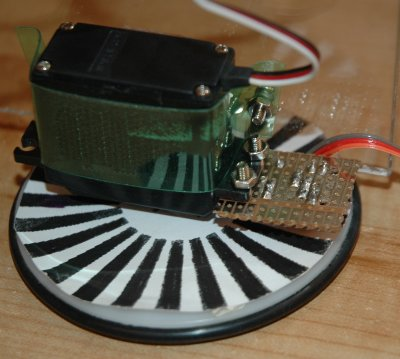
\includegraphics[width=0.6\linewidth]{encoders3}
            Home-made encoder

            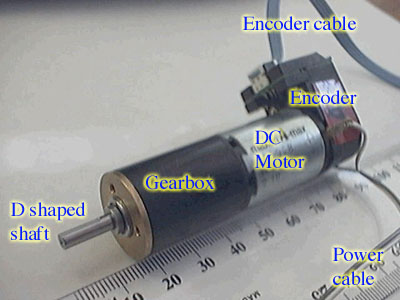
\includegraphics[width=0.6\linewidth]{encoders5}
            Commercial encoder

        \end{column}

        \begin{column}{0.5\linewidth}
            \centering

            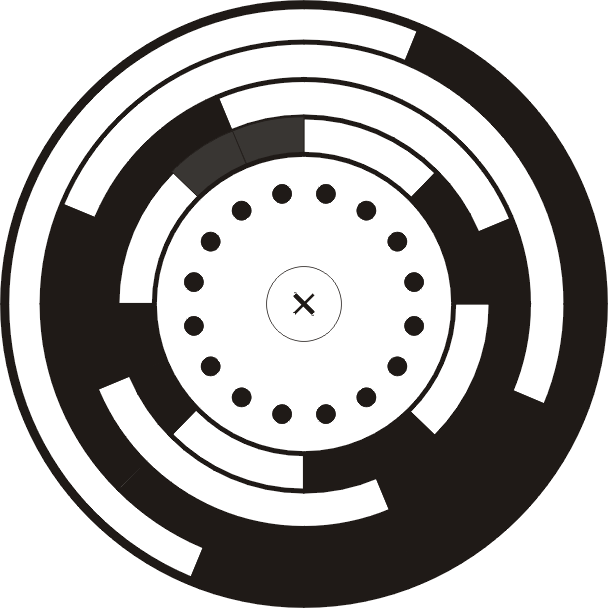
\includegraphics[width=0.9\linewidth]{encoders4}

            Absolute encoder disk
        \end{column}
    \end{columns}


\end{frame}

%%%%%%%%%%%%%%%%%%%%%%%%%%%%%%%%%%%%%%%%%%%%%%%%%%%%%%%%%%%%%%%%%%%%%%%%%%%%%%%%%%%%%%%%%%
\subsection{Heading}
\begin{frame}{Heading sensors}

    \begin{itemize}
        \item Heading sensors can be proprioceptive (gyroscope, inclinometer) or
              exteroceptive (compass).

        \item Used to determine the robots orientation and inclination.

        \item Allow, together with an appropriate velocity information, to integrate the
              movement to an position estimate. This procedure is called
              {\bf dead reckoning} (from ship navigation).

    \end{itemize}
\end{frame}

\begin{frame}{Compass}

    Since over 2000 B.C., when Chinese suspended a piece of naturally magnetite from a silk
    thread and used it to guide a chariot over land.

    Magnetic field on earth: {\bf absolute measure for orientation}

    Large variety of solutions to measure the earth magnetic field:
    \begin{itemize}
        \item mechanical magnetic compass
        \item direct measure of the magnetic field (Hall-effect, magnetoresistive
              sensors)
    \end{itemize}

    \emph{Major drawbacks}:

    \begin{itemize}
        \item weakness of the earth field
        \item easily disturbed by magnetic objects or other sources
        \item not feasible for indoor environments
    \end{itemize}

\end{frame}

\begin{frame}{Compass}

    Solid state compass, \eg Honeywell HMR3100:

    \begin{center}
        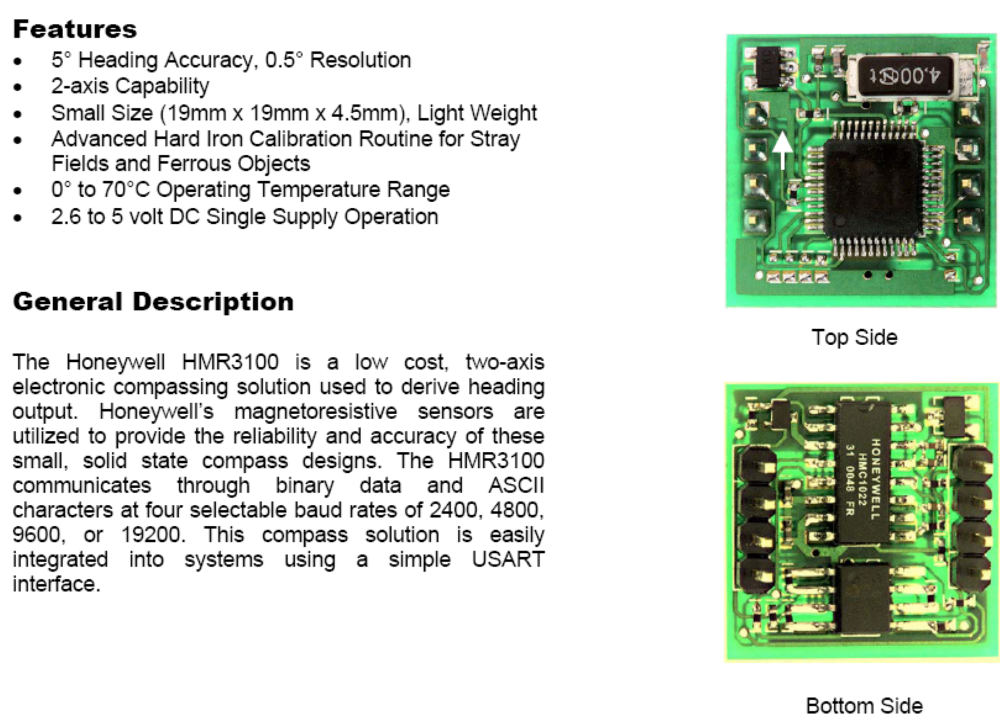
\includegraphics[width=0.8\linewidth]{compass}
    \end{center}
    \small
    \url{http://datasheet.digchip.com/197/197-01540-0-HMR3100.pdf}

\end{frame}

%%%%%%%%%%%%%%%%%%%%%%%%%%%%%%%%%%%%%%%%%%%%%%%%%%%%%%%%%%%%%%%%%%%%%%%%%%%%%%%%%%%%%%%%%%
\subsection{Gyroscopes}

\begin{frame}{Gyroscope}

    Reports an acceleration of rotation to a \textbf{relative frame of reference}.

    \textbf{Unlike a compass!} that keeps the orientation to a fixed frame: reference to an
    absolute frame of reference.

    \pause

    Two categories, the mechanical and the optical gyroscopes

    {\bf Mechanical Gyroscopes}

    \begin{itemize}
        \item Standard gyro
        \item Rated gyro
    \end{itemize}

    {\bf Optical Gyroscopes}

    \begin{itemize}
        \item Rated gyro
    \end{itemize}

\end{frame}

\begin{frame}{Mechanical gyroscopes}

    \begin{multicols}{2}
    \emph{Concept}: inertial properties of a fast spinning rotor $\Rightarrow$ \textbf{gyroscopic precession}

    Angular momentum associated with a spinning wheel keeps the axis of the
    gyroscope inertially stable.
        \vfill
        \columnbreak
        \video[0.82]{0.8\linewidth}{figs/gyro.mp4?autostart}
    \end{multicols}


    \only<1>{
    Reactive torque $\tau$ (tracking stability) is proportional to the
    spinning speed $\omega$, the precession speed $\Omega$ and the wheels
    inertia $\mathcal{I}$\bubblemark{inertia}.
    \[
        \tau = \mathcal{I}\cdot\omega\cdot\Omega
    \]
    \bubble<1>[30]{inertia}{$\mathcal{I} = \int_{W}r^2dm$}
    No torque can be transmitted from the outer pivot to the wheel axis: {\bf
    spinning axis will therefore be space-stable}
    }
    \only<2>{


        \emph{Quality}: 0.1° over 6 hours

    If the spinning axis is aligned with the north-south meridian, the
    earth's rotation has no effect on the gyro's horizontal axis

    If it points east-west, the horizontal axis reads the
    earth rotation
    }

\end{frame}

\imageframe[caption=Mechanical gyroscope of ballistic missile (French IRBM S3 -- 1970s -- Wikimedia)]{gyro-example}

\begin{frame}{Rate gyros}

    Same basic arrangement shown as regular mechanical gyros

    But: gimble(s) are restrained by a torsional spring

    \begin{beamercolorbox}{block body example}
        enables to measure angular speeds instead of the orientation.
    \end{beamercolorbox}

\end{frame}

\begin{frame}{Optical gyroscopes}

    \begin{multicols}{2}

        \begin{center}
            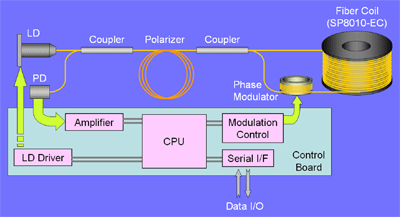
\includegraphics[width=0.9\linewidth]{optical-gyro}
        \end{center}

        \begin{center}
            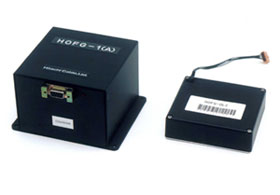
\includegraphics[width=0.7\linewidth]{optical-gyro2}
        \end{center}

        {\footnotesize Hitachi fibre optical gyroscope}

        \vfill
        \columnbreak

        First commercial use started only in the early 1980 when they where
        first installed in airplanes.

        Optical gyroscopes sensitive to only one plane. Report {\bf angular speed}
        instead of absolute orientation.


    \end{multicols}

\end{frame}

\begin{frame}{Optical gyros: Sagnac effect}

    \begin{multicols}{2}

        \only<1>{
        A beam of light is split, both beams follow a trajectory in opposite
        directions.


        One is traveling in a fiber clockwise, the other counterclockwise
        around a cylinder (older setups use a ring of mirrors).
        }

        \only<2>{
        Laser beam traveling in direction of rotation

        \begin{itemize}

            \item slightly shorter path \rightarrow shows a higher frequency
            \item difference in frequency $D_f$ of the two beams is proportional to the angular velocity $\omega$ of the cylinder
        \end{itemize}

        On return to the point of entry both beams form an {\bf interference
            pattern}. Rotating the apparatus results in a {\bf changing
        interference pattern}.
        }

        \vfill
        \columnbreak
    
        \vspace{2cm}
        \begin{center}
            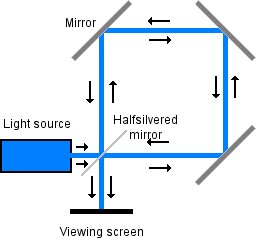
\includegraphics[width=0.8\linewidth]{sagnac-effect}
        \end{center}

    \end{multicols}
\end{frame}

\begin{frame}{Vibrating structure gyroscopes}

    A small vibrating element replaces the spinning wheel.

    \begin{itemize}

        \item {\bf Measures angular acceleration} (= rate gyroscope)
        \item {\bf Small} due to
            \href{http://en.wikipedia.org/wiki/Microelectromechanical_systems}{\bf
            MEMS} technology (\emph{Micro Electro Mechanical System}): lithographic
            etching of mechanical structure of mm (or smaller) size.

    \end{itemize}

    Many different ways of implementing this:

    \begin{itemize}

        \item Vibrating wheel gyroscope
        \item \href{http://en.wikipedia.org/wiki/Piezoelectric_effect}{Piezoelectric} element gyroscope
        \item Tuning forks manufactured using MEMS technology
        \item \ldots{}
    \end{itemize}

\end{frame}

\begin{frame}{Vibrating wheel gyroscope}

    Relies on gyroscopic effect, but executed in MEMS technology.

    \begin{center}
        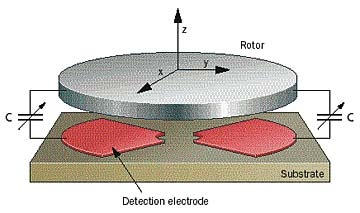
\includegraphics[width=0.4\linewidth]{vibratingwheel}\hspace{1em}
        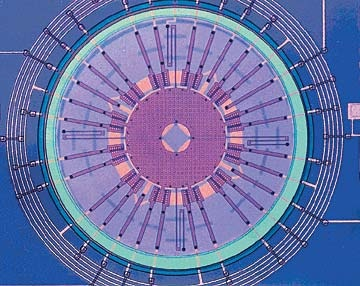
\includegraphics[width=0.4\linewidth]{vibratingwheel2}
        
        \bubblemark{wheel}\source{https://www.quora.com/How-does-a-MEMS-gyroscope-work}{Quora}

    \end{center}

    \bubble<1>[90][0.5cm][6cm]{wheel}{Wheel vibrates (equivalent to rotating), tilt due to gyropscopic effect
     change detected by change in capacitance}


\end{frame}

\begin{frame}{Technology: Coriolis effect}

    Mass $m$ moving in one direction at speed $\vec{v}$, when rotated at speed $\vec\Omega$,
    experiences a {\bf Coriolis} force $\vec{F}_{coriolis}$:

    \begin{center}
        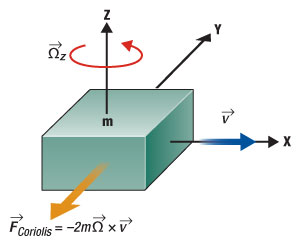
\includegraphics[width=0.5\linewidth]{coriolis}
        
        \source{http://electroiq.com/blog/2010/11/introduction-to-mems-gyroscopes/}{STM}
    \end{center}

    Displacement measured as \emph{change in capacitance}.



\end{frame}

\begin{frame}{Example}

    STMicroElectronics

    \begin{center}
        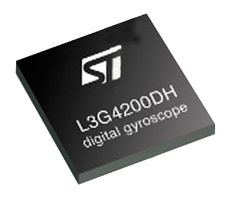
\includegraphics[width=0.3\linewidth]{stm_gyro}
    \end{center}

    \begin{itemize}

        \item
              low-power three-axis angular rate sensor
        \item
              I2C, SPI
        \item
              70 mdps sensitivity
        \item
              \href{http://www.st.com/web/en/resource/technical/document/datasheet/CD00265057.pdf}{Datasheet}
    \end{itemize}

    \small
    In depth information on gyroscopes see \url{http://ieee-sensors2013.org/sites/ieee-sensors2013.org/files/Serrano_Slides_Gyros2.pdf}

\end{frame}

\begin{frame}{Use of gyroscopes}

    \only<1>{
        Most gyroscopes return angular velocity: $rad\cdot s^{-1}$.

        Angular velocity can be converted to angle $a$ ({\it attitude} of the gyro) through integrating reading $\dot{a}$\bubblemark{derivative} over time:

        \[
            a = \int_{0}^{t} \dot{a}dt
        \]

        \bubble<1>[160][2.5cm][3cm]{derivative}{A variable with a dot on top is that variable at a particular point in time}

        \begin{multicols}{2}
            While classic optical or mechanical gyroscopes do not suffer from drift,
            MEMS gyroscopes do.
            
            Example, 30$^{\circ}$ drift over 12 sec!

            \begin{center}
                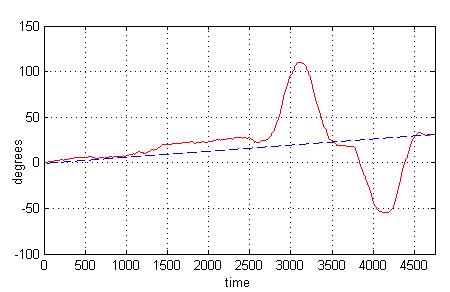
\includegraphics[width=0.8\linewidth]{gyro-drift}

                \source{http://tom.pycke.be/mav/70/gyroscope-to-roll-pitch-and-yaw}{Tom Pycke}
            \end{center}

        \end{multicols}

    }
    \only<2>{
        MEMS gyroscopes are very noisy:


        \begin{center}
            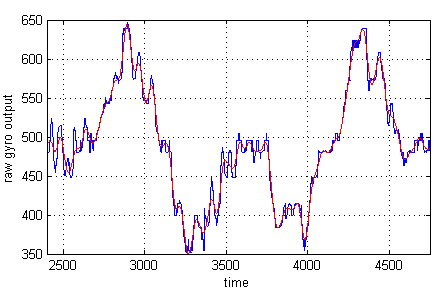
\includegraphics[width=0.6\linewidth]{mems-noise}\bubblemark{gyronoise}
        \end{center}
        Filtering needed to get rid of noise.
        \bubble<2>[180][0.3cm]{gyronoise}{Gyro rotates 90$^{\circ}$ clockwise and then 90$^{\circ}$ counter clockwise and back. Blue line is raw output from gyro, red is low pass filtered.}
    }
    \only<3>{


        {\bf Runge-Kutta filter}, implements a ``running average'', smoothing out
        the noise.

        \[
            a_t = a_{t-1} + \frac{1}{6}(\dot{a}_{t-3} + 2\dot{a}_{t-2} + 2\dot{a}_{t-1} + \dot{a}_t)
        \]

        \begin{center}
            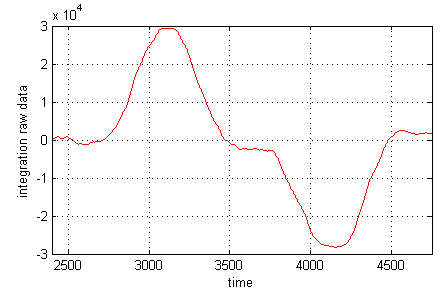
\includegraphics[width=0.6\linewidth]{mems-filtering}

            \source{http://tom.pycke.be/mav/70/gyroscope-to-roll-pitch-and-yaw}{Tom Pycke}
        \end{center}

    }
\end{frame}

%%%%%%%%%%%%%%%%%%%%%%%%%%%%%%%%%%%%%%%%%%%%%%%%%%%%%%%%%%%%%%%%%%%%%%%%%%%%%%%%%%%%%%%%%%
\subsection{Accelerometers}
\begin{frame}{Accelerometers}

    Accelerometers measure acceleration of the device

    \begin{itemize}

        \item Single axis: only measure a in one direction.
        \item Multi axis: measures in multiple direction, 3 axis is sufficient.
        \item Measured in $\frac{m}{s^2}$ or in $g = 9.81\cdot\frac{m}{s^2}$.
    \end{itemize}

    {\bf Principle}: damped mass on a spring; when mass accelerates,
    displacement is measured and translated to acceleration.

    \begin{multicols}{2}
        \begin{itemize}

            \item Modern accelerometers are MEMS

            \item Displacement is often indirectly measured using capacitive, peizoelectric
                  or \href{http://en.wikipedia.org/wiki/Piezoresistive_effect}{piezo\bubblemark{piezoresistive}resistive}
                  sensors.

                  \vfill
                  \columnbreak

        \end{itemize}

        \begin{center}
            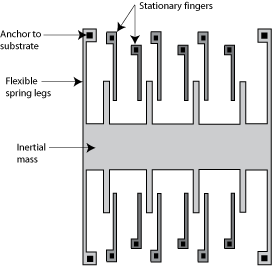
\includegraphics[width=0.6\linewidth]{accelero}

            \source{http://research.et.byu.edu/llhwww/intro/memsintro.html}{BYU}
        \end{center}
    \end{multicols}

    \bubble<1>[90][0.3cm][4.5cm]{piezoresistive}{Crystalline material changes resistance when under pressure}


\end{frame}

\begin{frame}{Accelerometer as tilt sensor}

    An accelerometer always senses the Earth's gravitational vector $\vec{g} = 9.81\cdot\frac{m}{s^2}$.

    As such an accelerometer can be used to \textbf{measure rotation}.

    \begin{itemize}
        \item Gravity vector will be sensed on all three axes as $\vec{g_x}$, $\vec{g_y}$, $\vec{g_z}$.

        \item The gravitation vector can be decomposed in three components, which
              need to vector sum to $\vec{g}$.

          \item However, it cannot measure rotation around the $\vec{z}$-axis, for that a
              gyroscope is still needed.

    \end{itemize}

    \begin{center}
        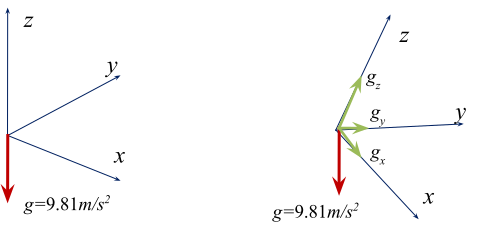
\includegraphics[width=0.5\linewidth]{accelero_tilt}
    \end{center}

\end{frame}

%%%%%%%%%%%%%%%%%%%%%%%%%%%%%%%%%%%%%%%%%%%%%%%%%%%%%%%%%%%%%%%%%%%%%%%%%%%%%%%%%%%%%%%%%%
\subsection{GPS}
\begin{frame}{Global Positioning System (GPS)}

    \only<1>{
        \begin{itemize}

            \item Developed for military use (since 1978)
            \item Cost of maintenance estimated at \$400M per year
            \item Recently it became accessible for commercial applications
            \item 24 satellites (excluding five spares) orbit the earth every 12 hours
                at a height of 20,190 km
            \item 4 satellites are located in each of six planes inclined 55$^{\circ}$
                with respect to the plane of the earth's equators
            \item From any location on the planet at least \textbf{4 satellites can be seen}
        \end{itemize}

    }
    \only<2>{

        \begin{center}
            \video[1]{6cm}{figs/gps.mp4?autostart}

            \source{https://en.wikipedia.org/wiki/File:GPS24goldenSML.gif}{Wikipedia}
        \end{center}
    }

\end{frame}

\begin{frame}{GPS - summary}

    \begin{itemize}

        \item Location of any GPS receiver is determined through a {\bf time of flight
            measurement}
            \item Two forms of clock information: {\bf Coarse/Acquisition} (C/A) code which is
                  public and {\bf Precise} code which is for military apps. The code also
                  carries the identifier of the satellite.
            \item Satellites carry {\bf high-precision atomic clocks}, while GPS receivers
                  have low precision crystal oscillator clocks (updated by the atomic
                  clocks)
        \end{itemize}

    \end{frame}

    \begin{frame}{GPS -- calculating position}

        \only<1> {
            \begin{itemize}

                \item
                      Suppose the time of flight to three satellites is known: $t_1$, $t_2$, $t_3$.
                \item
                      The distance to each satellite is $r_i = v_{air}\cdot t_i$
                \item
                      If the receivers position is $(x,y,z)$, and the satellites
                      position are $(x_i, y_i, z_i)$, the following relations hold:

                      \[
                          r_i = \sqrt{(x-x_i)^2 + (y - y_i)^2 + (z - z_i)^2}
                      \]
            \end{itemize}
        }

        \only<2>{

            Three spheres, intersection results in two solutions for $(x,y,z)$.
            One is above the earth's surface, the other below.

            \begin{center}
                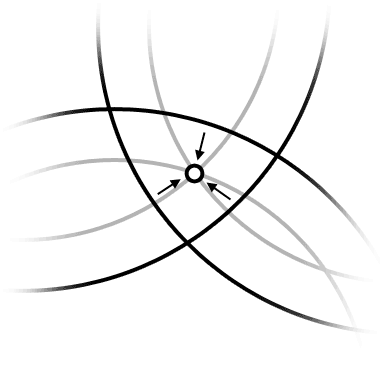
\includegraphics[width=0.3\linewidth]{gps_pos}
            \end{center}

        }
        \only<3>{


            \begin{exampleblock}{}
                A deviation in the receivers clock results an error on the distance to
                the satellite.
            \end{exampleblock}


            For example, for a satellite at 25,000km from the receiver, \emph{a 0.1ms deviation
            between clocks results in an error of 30m in the distance to the
            satellite}.
        }

        \only<4>{

            Assume the time difference between the atomic clocks and the receiver clock is
            $\Delta_t$. The distance to the satellites is now erroneously estimated
            at $r_i = v_{air}\cdot (t_i + \Delta_t)$

            $\Delta_t$ can be calculated by taking an extra satellite into account.

            \[
                r_1 = \sqrt{(x-x_1)^2 + (y - y_1)^2 + (z - z_1)^2} + K\cdot\Delta_t
            \]\[
            r_2 = \sqrt{(x-x_2)^2 + (y - y_2)^2 + (z - z_2)^2} + K\cdot\Delta_t
        \]\[
        r_3 = \sqrt{(x-x_3)^2 + (y - y_3)^2 + (z - z_3)^2} + K\cdot\Delta_t
    \]\[
    r_4 = \sqrt{(x-x_4)^2 + (y - y_4)^2 + (z - z_4)^2} + K\cdot\Delta_t
    \]

}
\end{frame}

\begin{frame}{GPS -- accuracy}

    With the C/A code, the time of flight can be measured to within 10ns,
    which is an error of $\approx$ 3m.

    Sources of error on the distance to satellite estimate:

    \begin{itemize}

        \item Time of flight measure accuracy: $\pm$ 3m
        \item Satellite clock errors: $\pm$ 2m
        \item Ephemeris errors (position of satellites): $\pm$ 2.5m
        \item \textbf<2>{Ionospheric effects} (signal dispersion): $\pm$ 5m
        \item \textbf<2>{Tropospheric effects} (dispersion due to humidity): $\pm$ 0.5m
        \item \textbf<2>{Multipath distortion} (reflections in environment): $\pm$ 1m
        \item Numerical errors $\pm$ 1m or less
    \end{itemize}

    $\Rightarrow$ {\bf typical accuracy is 15m}, but this varies a lot

\end{frame}

\begin{frame}{GPS - improvements}

    {\bf L1 and L2 frequency}

    Same time information is transmitted on two frequencies, these
    frequencies will experience noise in a different way. Can be used to
    cancel atmospheric noise.

    \pause

    {\bf Differential GPS (DGPS)}

    Stationary receiver, with known position, read GPS position and
    calculate the error. This error is broadcast over an FM band to
    receiver in the neighbourhood. Accuracy is 1 to 3 meters.

    \pause

    {\bf Satellite Based Augmentation System (SBAS)}

    Ground based receivers calculate ionospheric delays and clock drift,
    this is relayed to geosynchronous satellites which then broadcast it
    to all receivers in its view.

    The American FAA has a system which works
    in the Western hemisphere, called Wide Area Augmentation
    System~(WAAS).

\end{frame}

\begin{frame}{Galileo}

    Europe's response to GPS (or GLONASS, the Russian global positioning
    system).

    \begin{itemize}

        \item 30 spacecraft
        \item orbital altitude: 23,222 km
        \item 3 orbital planes, 56$^{\circ}$ inclination (9 operational satellites and one
              active spare per orbital plane)
        \item satellite lifetime: $>$12 years
    \end{itemize}

    \pause

    \begin{itemize}

        \item Free access: 1m accuracy
        \item Subscription access: up to 10cm accuracy
        \item Better high altitude positioning
    \end{itemize}

\end{frame}

\begin{frame}{GPS - Receivers}

    \begin{multicols}{2}

        {\bf Adafruit GPS Module - MTK3339 chipset}

        \begin{center}
            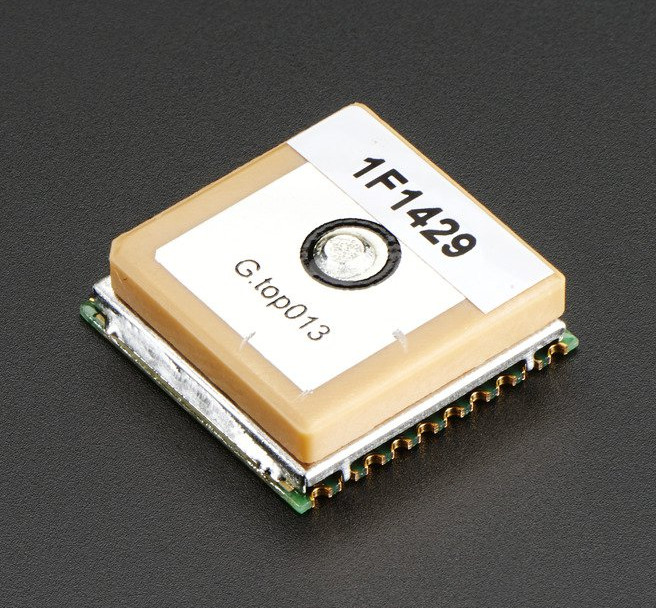
\includegraphics[width=0.8\linewidth]{adafruit_receiver}

            \source{https://www.adafruit.com/product/790}{Adafruit}
        \end{center}

        \vfill
        \columnbreak

        \begin{itemize}
            \item -165 dBm sensitivity, 10 Hz updates, \textbf<2-3>{66 channels}
            \item Ultra low power usage: 20mA current draw while tracking
            \item 3.3V operation,
            \item 16mm x 16mm x 5mm and 4 grams
            \item $\approx$ £23
        \end{itemize}

        \only<2>{
            {\bf Why 66 channels when only max. 12 satellites are visible?}
        }
        \only<3>{
            \href{http://electronics.stackexchange.com/a/11900}{Improved correlation time} $\rightarrow$ faster acquisition; lower power consumption
        }
        \vfill

    \end{multicols}

\end{frame}

\begin{frame}{GPS -- Applications in robotics}

    GPS only works \textbf{outdoors}

    \begin{itemize}

        \item
              Due to limited energy (--163 dBw~or 5 x 10--17~watts) and high
              frequency (1.57542~GHz for L1 signal and 1.2276~GHz for L2 signal) of
              signal, GPS packets do not penetrate buildings.
    \end{itemize}

    Limited accuracy

    \begin{itemize}

        \item Accuracy several meters up to tens of meters. Autonomous vehicles will
              need to rely on other localisation methods.
    \end{itemize}

    \pause

    \begin{multicols}{2}

        \vfill
        Accuracy can be dramatically improved using a local DGPS antenna.

        \vfill
        \columnbreak
        \begin{center}
            \video{5cm}{figs/dgps_demo.webm?start=13}\\
            \source{http://www.youtube.com/watch?v=FATVNEB1_BY}{youtube}
        \end{center}

    \end{multicols}
\end{frame}

\begin{frame}{GPS -- Examples}
    \begin{multicols}{2}

        Positioning of outdoor service robots

        \begin{center}
            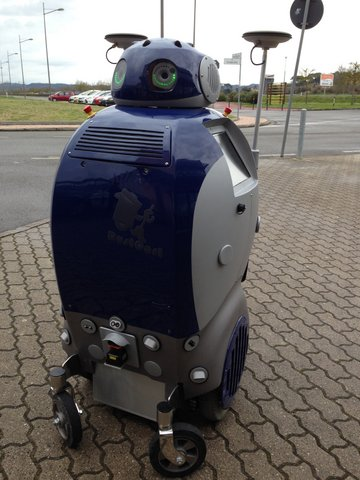
\includegraphics[width=0.8\linewidth]{gps-example1}\\
            \source{http://www.robotera.eu/}{www.robotera.eu}
        \end{center}

        \columnbreak
        Agricultural robots


        \begin{center}
            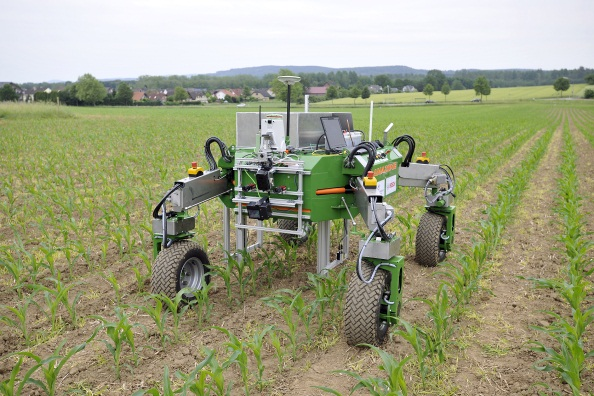
\includegraphics[width=0.9\linewidth]{gps-example2}
        \end{center}

        Sowing, weeding, harvesting with cm precision
    \end{multicols}

\end{frame}

%%%%%%%%%%%%%%%%%%%%%%%%%%%%%%%%%%%%%%%%%%%%%%%%%%%%%%%%%%%%%%%%%%%%%%%%%%%%%%%%%%%%%%%%%%
\subsection{Other radio localisation methods}

\begin{frame}{Other radio localisation methods}

    Mainly used in mobile phones and mobile devices

    \textbf{GSM-based triangulation}

    \begin{itemize}

        \item
              Uses strength of GSM signal of different GSM base stations to estimate
              position
        \item
              Works indoors, but accuracy limited to a radius of about 1km
    \end{itemize}

    \pause

    \textbf{WiFi-based localisation}

    \begin{itemize}
        \item
              Whenever a device connects to a WiFi router, it knows the IP of the
              router. Some Internet providers know at which address a router is and
              provide this (\emph{geo-coding})
        \item When available, more accurate as range of WiFi router is limited, radius of about 50m.
        \item Alternatively, positioning via databases that associate unique IDs (MAC
              addresses) of WiFi routers with their location. For example,
              \href{https://location.services.mozilla.com/}{Mozilla Location Service}

    \end{itemize}

\end{frame}

\imageframe[caption=Regions covered by Mozilla Location Service, color=black]{mozilla-localisation}

%%%%%%%%%%%%%%%%%%%%%%%%%%%%%%%%%%%%%%%%%%%%%%%%%%%%%%%%%%%%%%%%%%%%%%%%%%%%%%%%%%%%%%%%%%
\subsection{Range sensors}

\begin{frame}{Range sensors (time of flight)}

    \only<1>{

        Large range distance measurement \rightarrow {\bf range sensors}

        Range information: key element for {\bf localisation} and {\bf environment modeling}

        Ultrasonic sensors as well as laser range sensors make use of propagation speed
        of sound or electromagnetic waves respectively. The traveled distance of a
        sound or electromagnetic wave is given by $d = c \cdot t$, where:

        \begin{itemize}

            \item
                  $d$: distance traveled (usually round-trip)
            \item
                  $c$: speed of wave propagation
            \item
                  $t$: time of flight
        \end{itemize}
    }

    \only<2>{
        It is important to point out that:

        \begin{itemize}
            \item Propagation speed $\nu$ of sound: $0.3 \frac{m}{ms}$
            \item Propagation speed $\nu$ of of electromagnetic signals: $0.3 \frac{m}{ns}$ \\
                  $\Rightarrow$ one million times faster
        \end{itemize}

        \pause

        3 meters is:

        \begin{itemize}

            \item
                  10 ms for an ultrasonic system
            \item
                  only 10 ns for a laser range sensor
        \end{itemize}

        Measuring the time of flight $t$ with electromagnetic signals is \textbf{not an easy task}; laser range sensors are expensive and delicate

    }

    \only<3>{

        The quality of time of flight range sensors mainly depends on:

        \begin{itemize}

            \item Uncertainties about the exact time of arrival of the reflected signal,
                  due to reflections, multiple echos, \ldots{}
            \item Internal sensor inaccuracies in the time of flight measure (laser
                  range sensors)
            \item Opening angle of transmitted beam (ultrasonic range sensors)
            \item Interaction with the target (surface, specular reflections)
            \item Variation of propagation speed
            \item Speed of mobile robot and target (if not at standing still)
        \end{itemize}
    }

\end{frame}

\begin{frame}{Ultrasonic Sensor (sonar)}


    \only<1>{

    Transmit a packet of (ultrasonic) pressure waves.

    The distance $d$ of the echoing object can be calculated based on the
    propagation speed of sound $c$ and the time of flight $t$:
    \[
        d = \frac{c_{gas}\cdot t}{2}
    \]

    The speed of sound $c_{gas}$ in a gas is given by:
    \[
        c_{gas} = \sqrt{g\cdot R\cdot T}
    \]

    where:

    \begin{itemize}
        \item  $g$: adiabatic index, 1.40 for air
        \item $R$: gas constant, 287.053072 $\frac{J}{kg\cdot K}$ for air
        \item $T$: temperature in degree Kelvin

    \end{itemize}

    }
    \only<2>{

    The speed of sound in air can be approximated by:
    \[
        c_{air} = 331.3 \sqrt{1+\frac{J}{273.15}}
    \]
    with $J$ the air temperature in Celsius.

    If no correction for temperature would be done, what would the error be?

        Assume obstacle at 1m, and $T = 15^{\circ}C$:

        \centering
        \begin{tabular}{@{}llll@{}}
            \toprule
            T ($^{\circ}C)$ & $c$   & $t$     & \bf Error (\%) \\ \midrule
            -10          & 325.2 & 0.00615 & \bf 4.6        \\
            0            & 331.3 & 0.00604 & \bf 2.7        \\
            15           & 340.3 & 0.00588 & \bf 0          \\
            30           & 349.0 & 0.00573 & \bf -2.5       \\ \bottomrule
        \end{tabular}

    }

\end{frame}

\begin{frame}[plain]

    \centering
    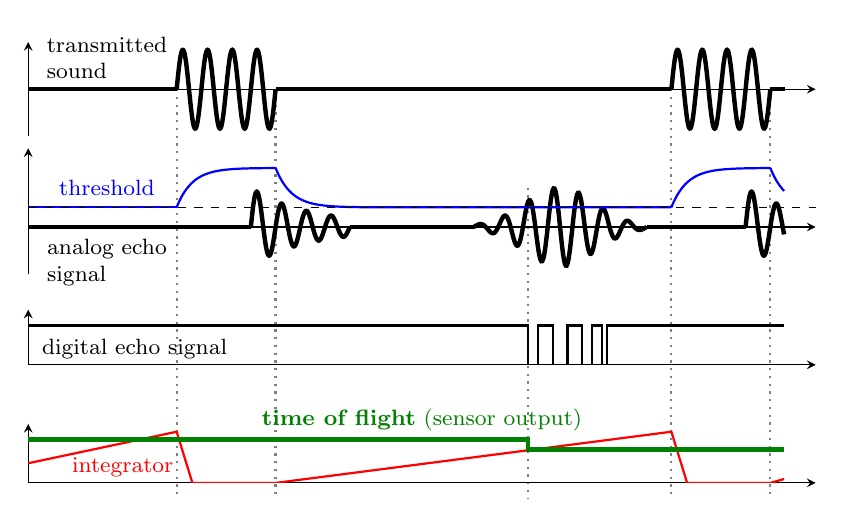
\begin{tikzpicture} 
        [label/.style={align=left,font=\footnotesize}]

        \draw[dotted,thick, gray] (3*pi * 0.2 ,0) -- (3*pi * 0.2, -5.2);
        \draw[dotted,thick, gray] (5*pi * 0.2 ,0) -- (5*pi * 0.2, -5.2);
        \draw[dotted,thick, gray] (13*pi * 0.2 ,0) -- (13*pi * 0.2, -5.2);
        \draw[dotted,thick, gray] (15*pi * 0.2 ,0) -- (15*pi * 0.2, -5.2);

        \draw[dotted,thick, gray] (10.1*pi * 0.2 ,-2.5*0.5) -- (10.1*pi * 0.2, -5.2);


        \begin{axis}[
                anchor=origin,
            at={(0,0)},
            disabledatascaling,
            x=2mm,y=5mm,
            ticks=none, no markers, domain=0:50, samples=200,
            axis x line=middle,
            axis y line=left,
            height=5cm, width=\linewidth,
            ymin=-1.2,ymax=1.2,
            xmin=0,xmax=50,
        ]
            \addplot[ultra thick,domain=0:3*pi] {0}; 
            \addplot[ultra thick,domain=3*pi:5*pi] {sin(deg(4*x))}; 
            \addplot[ultra thick,domain=5*pi:13*pi] {0}; 
            \addplot[ultra thick,domain=13*pi:15*pi] {sin(deg(4*x))}; 
            \addplot[ultra thick,domain=15*pi:48] {0}; 
        \end{axis}

        \node[label] at (1,0.4) {transmitted \\ sound};

        \begin{axis}[
                anchor=origin,
            at={(0,-3.5)},
            disabledatascaling,
            x=2mm,y=5mm,
            ticks=none, no markers, domain=0:50, samples=200,
            axis x line=middle,
            axis y line=left,
            height=5cm, width=\linewidth,
            ymin=-1.2,ymax=2,
            xmin=0,xmax=50,
        ]

            \addplot[ultra thick,domain=0:4.5*pi] {0}; 
            \addplot[ultra thick,domain=4.5*pi:6.5*pi] {sin(deg(4*(x-1.5*pi)))/(x/(4.5*pi))^4}; 
            \addplot[ultra thick,domain=6.5*pi:9*pi] {0}; 

            \addplot[ultra thick,domain=9*pi:12.5*pi] {sin(deg(4*(x)))* exp(-(x-10.75*pi)^2/10)}; 

            \addplot[ultra thick,domain=12.5*pi:14.5*pi] {0}; 
            \addplot[ultra thick,domain=14.5*pi:48] {sin(deg(4*(x-1.5*pi)))/((x-10*pi)/(4.5*pi))^4}; 

            \addplot[thick,blue,domain=0:3*pi] {0.5};
            \addplot[thick,blue,domain=3*pi:5*pi] {1-exp(-x+3*pi) + 0.5}; 
            \addplot[thick,blue,domain=5*pi:13*pi] {exp(-x+5*pi) + 0.5}; 
            \addplot[thick,blue,domain=13*pi:15*pi] {1-exp(-x+13*pi) + 0.5}; 
            \addplot[thick,blue,domain=15*pi:48] {exp(-x+15*pi) + 0.5}; 
        \end{axis}

        % threshold
        \node[label,blue] at (1,-1.25) {threshold};
        \draw[dashed] (0 , -3 * 0.5) -- (50 * 0.2, -3 * 0.5);
        \node[label] at (1,-2.2) {analog echo \\ signal};


        \begin{axis}[
                anchor=origin,
            at={(0,-7)},
            disabledatascaling,
            x=2mm,y=5mm,
            ticks=none, no markers, domain=0:50, samples=200,
            axis x line=middle,
            axis y line=left,
            height=5cm, width=\linewidth,
            ymin=0,ymax=1.4,
            xmin=0,xmax=50,
        ]

            \addplot[thick] coordinates {
                (      0, 1)
                (10.1*pi, 1)
                (10.1*pi, 0)
                (10.3*pi, 0)
                (10.3*pi, 1)
                (10.6*pi, 1)
                (10.6*pi, 0)
                (10.9*pi, 0)
                (10.9*pi, 1)
                (11.2*pi, 1)
                (11.2*pi, 0)
                (11.4*pi, 0)
                (11.4*pi, 1)
                (11.6*pi, 1)
                (11.6*pi, 0)
                (11.7*pi, 0)
                (11.7*pi, 1)
                (     48, 1)
            };
        \end{axis}

        \node[label] at (1.35,-3.3) {digital echo signal};

        \begin{axis}[
                anchor=origin,
            at={(0,-10)},
            disabledatascaling,
            x=2mm,y=5mm,
            ticks=none, no markers, domain=0:50, samples=10,
            axis x line=middle,
            axis y line=left,
            height=5cm, width=\linewidth,
            ymin=0,ymax=1.5,
            xmin=0,xmax=50,
        ]
            \addplot[thick,red] coordinates {
                (0, 0.5)
                (3*pi, 1.3)
                (3*pi + 1, 0)
                (5*pi, 0)
                (13*pi, 1.3)
                (13*pi + 1, 0)
                (15*pi, 0)
                (48, 0.1)
            };
            \addplot[ultra thick,green!50!black] coordinates {
                (0, 1.1)
                (10.1*pi, 1.1)
                (10.1*pi, 0.85)
                (48, 0.85)
            };
        \end{axis}

        \node[label,red] at (1.2,-4.8) {integrator};
        \node[label,green!50!black] at (5,-4.2) {{\bf time of flight} (sensor output)};

    \end{tikzpicture}

    \source{https://books.google.co.uk/books?id=4of6AQAAQBAJ&pg=PA127}{Autonomous Mobile Robots, p.127}
\end{frame}

\begin{frame}{Ultrasonic sensor properties}

    \begin{itemize}
        \item Typical frequency: \textbf{40 -- 180 kHz}
        \item Generation of sound wave: piezo transducer
        \item Transmitter and receiver: same unit or separate units (for reduced \emph{blanking time})
    \end{itemize}

    Sound beam propagates in a cone-like manner:

    \begin{itemize}
        \item opening angles around 20 to 40 degrees
        \item acquisition of \emph{regions of constant depth} rather than depth
            points $\rightarrow$ segments of an arc (sphere for 3D)
    \end{itemize}

\end{frame}

\begin{frame}{Problems with reflection}

    \begin{itemize}

        \item Soft surfaces absorb most of the acoustic energy
        \item Surfaces that are far from being perpendicular to the direction of
              the sound: specular reflection
    \end{itemize}

    \begin{center}
        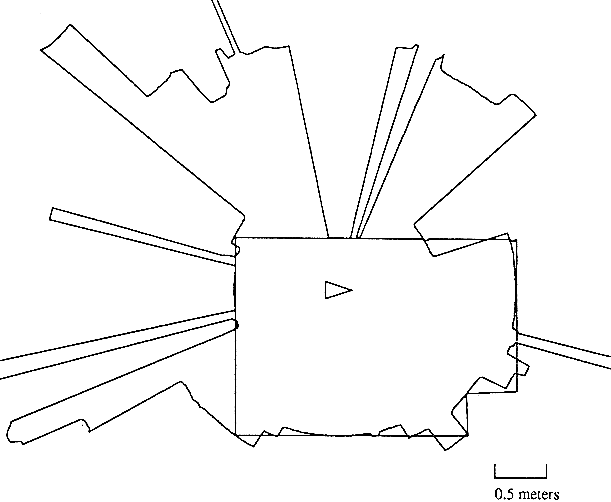
\includegraphics[width=0.6\linewidth]{us_scan}

        \source{https://books.google.co.uk/books?id=4of6AQAAQBAJ&pg=PA129}{Autonomous Mobile Robots, p.129}
    \end{center}
\end{frame}

\begin{frame}{Cycle time of ultrasonic sensors}

    When emitter and receiver are one and the same piece of hardware, the
    sensor has a \textbf{blanking time}.

    \begin{itemize}
        \item Time after the ping in which the sensor is blind
        \item Close obstacles will be missed
    \end{itemize}

    \textbf{Cycle time} is rather low

    \begin{itemize}
        \item In a moderately sized room where obstacles are 3m away, the time of
              flight is about 20ms. The sensor refresh rate is 50Hz.
        \item However, if a ring of sonar sensors is used, only one sensor at a time
              can be fired. For example, a 20 sensor ring will only operate at
              2.5Hz.
    \end{itemize}

\end{frame}

\begin{frame}{Sonar sensors}

    \begin{columns}
        \begin{column}{0.6\linewidth}

            LV-MaxSonar

            \begin{itemize}
                \item \url{http://www.maxbotix.com/}
                \item Detect 0 to 6.5m, range sensing 0.2 to 6.5m
                \item 42 kHz sonar ping.
                \item Serial out.
                \item Free run or triggered.
                \item \$25 - \$30
            \end{itemize}

        \end{column}
        \begin{column}{0.4\linewidth}

            \begin{center}
                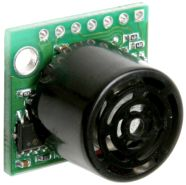
\includegraphics[width=0.8\linewidth]{maxbotix-lvmax}
            \end{center}
        \end{column}
    \end{columns}
\end{frame}

\begin{frame}{Laser Range Sensor}
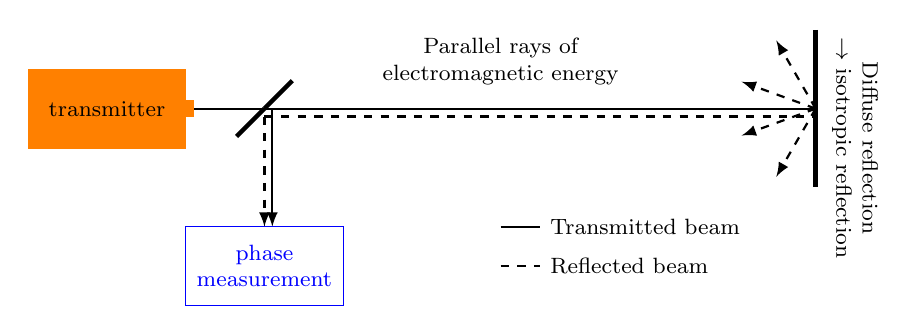
\begin{tikzpicture} 
    [>=latex,label/.style={align=center,font=\footnotesize}]

    \draw[thick] (2, 0.5) -- (10, 0.5);
    \draw[fill,orange] (0,0) rectangle (2,1);
    \draw[fill,orange] (1.9,0.4) rectangle (2.1,0.6);
    \draw[thick, dashed] (3, 0.4) -- (10, 0.4);
    \draw[thick, dashed,->] (10, 0.5) -- +(160:1);
    \draw[thick, dashed,->] (10, 0.5) -- +(120:1);
    \draw[thick, dashed,->] (10, 0.5) -- +(200:1);
    \draw[thick, dashed,->] (10, 0.5) -- +(240:1);

    \draw[ultra thick] (10, 1.5) -- +(0,-2);
    \draw[ultra thick] (3, 0.5) -- +(45:0.5);
    \draw[ultra thick] (3, 0.5) -- +(225:0.5);

    \draw[thick, dashed,->] (3, 0.4) -- (3, -1);
    \draw[thick, ->] (3.1, 0.5) -- (3.1, -1);

    \draw[blue] (2,-1) rectangle (4,-2);

    \node[label,blue] at (3,-1.5) {phase\\measurement};
    \node[label] at (1,0.5) {transmitter};

    \draw[thick] (6,-1) -- (6.5,-1) node[label,right] {Transmitted beam};
    \draw[thick,dashed] (6,-1.5) -- (6.5,-1.5) node[label,right] {Reflected beam};

    \node[label] at (6,1.1) {Parallel rays of \\electromagnetic energy};

    \node[label,rotate=-90] at (10.5,0) {Diffuse reflection\\$\rightarrow$ isotropic reflection};

\end{tikzpicture}

    \begin{itemize}
        \item Transmitted and received beams coaxial
        \item Transmitter illuminates a target with a collimated beam
        \item Receiver detects the time needed for round-trip
        \item A mechanical mechanism with a mirror sweeps
        \begin{itemize}
            \item 2D or 3D measurement
        \end{itemize}
    \end{itemize}

\end{frame}

\begin{frame}{Measuring time of flight: Phase-shift measurement}

    \only<1>{
    \begin{itemize}
        \item \emph{Pulsed laser}: same principle as ultrasonic sonar
        \item measurement of elapsed time directly
        \item \textbf{need to resolve picoseconds!} \rightarrow expensive hardware.
    \end{itemize}


    \begin{itemize}
        \item \emph{Indirect measure}: the time of flight measured using a \textbf{phase shift}
    measurement to produce range estimation.

        \item technically easier than the above two methods.
    \end{itemize}

}
    \only<2-5>{

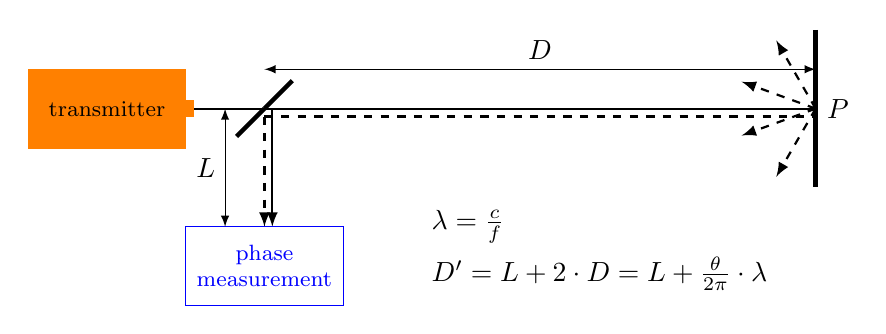
\begin{tikzpicture} 
    [>=latex,label/.style={align=center,font=\footnotesize}]

    \draw[thick] (2, 0.5) -- (10, 0.5);
    \draw[fill,orange] (0,0) rectangle (2,1);
    \draw[fill,orange] (1.9,0.4) rectangle (2.1,0.6);
    \draw[thick, dashed] (3, 0.4) -- (10, 0.4);
    \draw[thick, dashed,->] (10, 0.5) -- +(160:1);
    \draw[thick, dashed,->] (10, 0.5) -- +(120:1);
    \draw[thick, dashed,->] (10, 0.5) -- +(200:1);
    \draw[thick, dashed,->] (10, 0.5) -- +(240:1);

    \draw[ultra thick] (10, 1.5) -- +(0,-2) node[right,midway] {$P$};
    \draw[ultra thick] (3, 0.5) -- +(45:0.5);
    \draw[ultra thick] (3, 0.5) -- +(225:0.5);

    \draw[thick, dashed,->] (3, 0.4) -- (3, -1);
    \draw[thick, ->] (3.1, 0.5) -- (3.1, -1);

    \draw[blue] (2,-1) rectangle (4,-2);

    \node[label,blue] at (3,-1.5) {phase\\measurement};
    \node[label] at (1,0.5) {transmitter};

    \draw[<->] (2.5,0.5) -- (2.5,-1) node[left,midway] {$L$};
    \draw[<->] (3,1) -- (10,1) node[above,midway] {$D$};

    \node[align=left, anchor=west] at (5,-1) {$\lambda = \frac{c}{f}$};
    \node[align=left, anchor=west] at (5,-1.6) {$D' = L + 2\cdot D = L + \frac{\theta}{2 \pi} \cdot \lambda$};

\end{tikzpicture}
    }

    \vspace{1em}

    \only<2-3>{

        \begin{columns}
            \begin{column}{0.5\linewidth}
    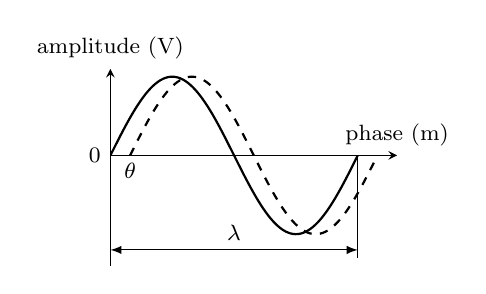
\begin{tikzpicture} 
        [>=latex,label/.style={align=left,font=\footnotesize}]

        \begin{axis}[
            anchor=origin,
            at={(0,0)},
            disabledatascaling,
            x=0.5cm,y=1cm,
            ticks=none,no markers, samples=100,
            axis x line=middle,
            axis y line=left,
            height=4cm, width=5cm,
            ymin=-1.4,ymax=1.1,
            xmin=0, xmax=2*pi+1
        ]
            \addplot[thick,domain=0:2*pi] {sin(deg(x))}; 
            \addplot[thick,dashed,domain=0.5:2*pi + 0.5] {sin(deg(x-0.5))}; 
        \end{axis}

        \draw[<->] (0,-1.2) -- (pi,-1.2) node[label,above,midway] {$\lambda$};
        \draw (pi, 0) -- (pi,-1.3);
        \node[label] at(-0.2,0) {0};
        \node[label] at(0.25,-0.2) {$\theta$};
        \node[label,anchor=south] at(0,1.1) {amplitude (V)};
        \node[label,anchor=south] at(pi + 0.5,0) {phase (m)};
\end{tikzpicture}

            \end{column}
            \begin{column}{0.5\linewidth}
    \only<2>{
        where $c$ is the speed of light; $f$ the
        modulating frequency; $D'$ the total distance covered by the emitted light;
        $\theta$ the (measured) phase shift.
    }
    \only<3>{

        \[
        \Rightarrow D = \frac{\lambda}{4\pi}\theta
        \]
    }
            \end{column}
        \end{columns}

    }
    \only<4>{

        For $f$ = 5 Mhz, $\lambda$ = 60 meters.

        Theoretically, \emph{ambiguous range estimates} are possible. For example if
        $\lambda$ = 60m, a target at a range of 5m $\equiv$ target at 35m (same
        $\theta$).

        Usually not an issue as the range of the sensor is typically smaller
        than $\lambda$ due to attenuation.
    }
    \only<5>{

        Confidence in the range (phase estimate) is \emph{inversely
        proportional to the square of the received signal amplitude}.

        Hence \emph{dark, distant objects will not produce such good range
        estimates} as closer brighter objects \ldots{}

    }
\end{frame}

\imageframe[color=black,caption=The sensors point down to avoid ambiguities]{darpa-urban-challenge}

\begin{frame}{Mechanical implementation}

    \begin{columns}
        \begin{column}{0.5\linewidth}
            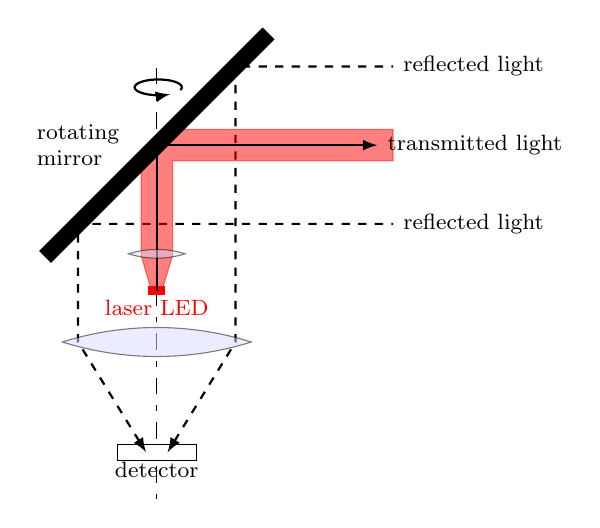
\begin{tikzpicture} 
                [>=latex,label/.style={align=left,font=\footnotesize}]

                \pgfmathsetmacro{\lensRadius}{4}
                \pgfmathsetmacro{\lensHeight}{1.2}
                \pgfmathsetmacro{\startAngle}{asin(\lensHeight/\lensRadius)}

                \draw[dash pattern=on 2pt off 4pt on 6pt off 4pt] (0,-1.5) -- (0,4);
                \draw[thick,->] (0.3,3.7) arc[start angle=-20, end angle=300,x radius=0.3, y radius=0.1];
                \filldraw[fill=white] (-0.5,-1) rectangle (0.5, -0.8) node[label,below,midway] (detector) {detector};
                \draw[thick,dashed,<-] (detector) -- (-1,0.5) -- (-1,2) -- (3,2) node[label,anchor=west] {reflected light};
                \draw[thick,dashed,<-] (detector) -- (1,0.5) -- (1,4) -- (3,4) node[label,anchor=west] {reflected light};
                \filldraw[red] (-0.1,1.1) rectangle (0.1, 1.2) node[label,below,midway] (led) {laser LED};
                \filldraw[red, semitransparent] (led) -- (-0.2,1.6) -- (-0.2,2.9) -- (0.2,3.2) -- (3,3.2) -- (3,2.8) -- (0.2,2.8) -- (0.2,1.6) -- (led);
                \draw[thick,black,->] (led) -- (0,3) -- (2.8,3) node[label,anchor=west] {transmitted light};
                \filldraw[black,rotate around={45:(0,3)}] (-2,3.1) rectangle (2,2.9);

                \node[label] at (-1,3) {rotating\\mirror};

                \draw [rotate=90,fill=blue!15, semitransparent]  (0.5,\lensHeight)
                arc[start angle=180-\startAngle,delta angle=2*\startAngle,radius=\lensRadius]
                arc[start angle=-\startAngle,delta angle=2*\startAngle,radius=\lensRadius]
                -- cycle; % to get a better line end

                \draw [rotate=90,scale=0.3,fill=blue!15, semitransparent]  (5.4,\lensHeight)
                arc[start angle=180-\startAngle,delta angle=2*\startAngle,radius=\lensRadius]
                arc[start angle=-\startAngle,delta angle=2*\startAngle,radius=\lensRadius]
                -- cycle; % to get a better line end

            \end{tikzpicture}

        \end{column}
        \begin{column}{0.5\linewidth}

            \begin{center}
                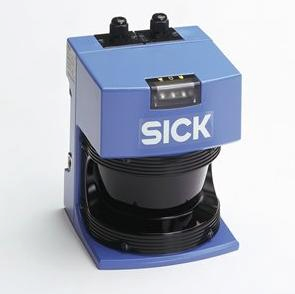
\includegraphics[width=0.6\linewidth]{SICK_LMS200}

                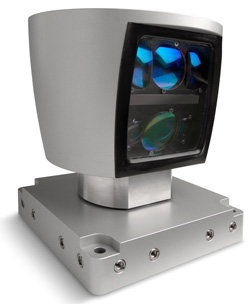
\includegraphics[width=0.6\linewidth]{velodyne}
            \end{center}
        \end{column}
    \end{columns}

\end{frame}

\begin{frame}{2D laser scan}

    Typical range image of a 2D laser range sensor with a rotating mirror.
    The length of the lines through the measurement points indicate the
    uncertainties.

    \begin{center}
        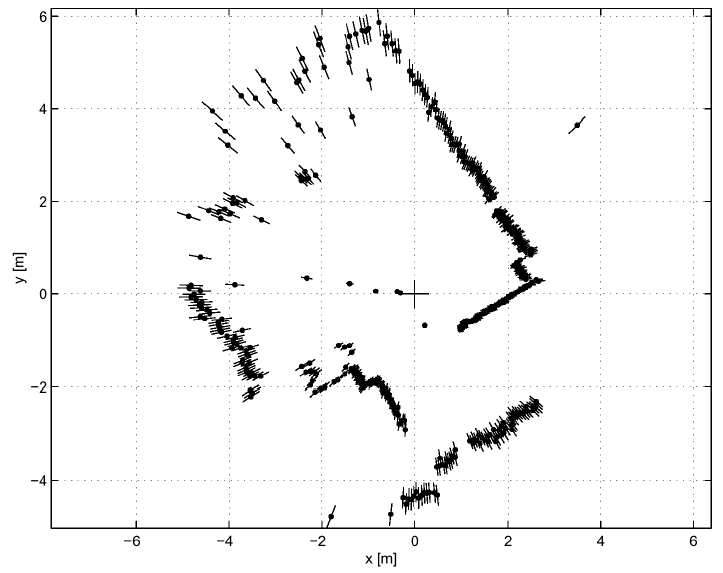
\includegraphics[width=0.7\linewidth]{laserscan}
    \end{center}
\end{frame}

\begin{frame}{Laser range finder}

    \begin{columns}
        \begin{column}{0.5\linewidth}
    \textbf{Hokuyo UST-10LX}

    \begin{itemize}

        \item 270° field of view.
        \item 0.25° angular resolution.
        \item 40 Hz scan rate.
        \item Ethernet
        \item Range 20mm to 10m $\pm$ 40mm
        \item Dimensions: 50 x 50 x 70mm
        \item Power: 0.15A 24V
        \item \$1775 in 2016
    \end{itemize}

            \source{https://acroname.com/products/HOKUYO-UST-10LX-LASER}{acroname}
            
        \end{column}
        \begin{column}{0.5\linewidth}
            \begin{center}
                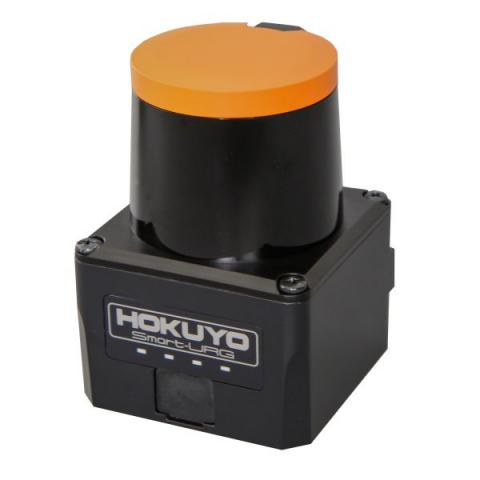
\includegraphics[width=0.8\linewidth]{hokuyo}
            \end{center}
        \end{column}
    \end{columns}

\end{frame}

\begin{frame}{Triangulating distance sensor}
    \textbf{Principle of 1D laser triangulation}
    \begin{tikzpicture} 
        [>=latex,label/.style={align=center,font=\footnotesize}]

        \pgfmathsetmacro{\lensRadius}{3}
        \pgfmathsetmacro{\lensHeight}{1}
        \pgfmathsetmacro{\startAngle}{asin(\lensHeight/\lensRadius)}
    
        \only<1>{
        \coordinate (target) at (10,0.5);
        }
        \only<2>{
        \coordinate (target) at (7,0.5);
        }

        \coordinate (lens) at (3.2,-1);
        \coordinate (psd) at (1.5,-1);
        \coordinate (psd2) at ($(psd) + (0,-1.5)$);

        \coordinate (impact) at (intersection of target--lens and psd--psd2);

        \fill [red, opacity=0.5] (impact) circle (2pt);

        \draw[thick] (2, 0.5) -- (target);

        \draw[fill,orange] (0,0) rectangle (2,1);
        \draw[fill,orange] (1.9,0.4) rectangle (2.1,0.6);
        \node[label] at (1,0.5) {transmitter};

        \draw[thick, dashed,->] (target) -- +(160:1);
        \draw[thick, dashed,->] (target) -- +(120:1);
        \draw[thick, dashed,->] (target) -- +(200:1);
        \draw[thick, dashed,->] (target) -- +(240:1);

        \draw[ultra thick] (target)++(0, 1) -- ++(0,-2) node[right,midway] {$P$};

        \draw[thick, dashed,->] (target) -- (impact);

        \draw[<->] (2.5,0.5) -- (2.5,1 |- psd) node[left,midway] {$L$};

        \draw[<->] (lens |- 0,1) -- (target |- 0,1) node[above,midway] {$D$};
        \draw ($(lens) + (0,1.1)$) -- (lens |- 0,1.1);

        \draw ($(psd) + (-1,0)$) -- ($(psd) + (1.2,0)$);
        \draw[thick] (psd) rectangle ($(psd2)+(-0.3,0)$);
        \foreach \a in {0.1,0.2,...,1.5}
            \draw ($(psd) + (0,-\a)$) -- +(-0.3,0);

        \node[label,anchor=north] at (1.5,-2.5) {Position-Sensitive Device (PSD) \\ or Linear Camera};

        \draw (impact -| 0.5,0) -- +(0.5,0);
        \draw[<->] (impact -| 0.6,0) -- (0.6,-1 |- psd) node[left,midway] {$x$};

        \draw [fill=blue!15, semitransparent]  ($(lens)+(0,\lensHeight)$)
        arc[start angle=180-\startAngle,delta angle=2*\startAngle,radius=\lensRadius]
          arc[start angle=-\startAngle,delta angle=2*\startAngle,radius=\lensRadius]
             -- cycle;

        \draw[<->] (psd |- 0,-2.1) -- (lens |- 0,-2.1) node[below,midway] {$f$};

        \node[label,anchor=west] at (3.2,-2) {Lens};

        \node[align=left, anchor=west] at (5,-2) {$D = f\cdot \frac{L}{x}$};

    \end{tikzpicture}

    \onslide<2>{
       Note that distance is proportional to $\frac{1}{x}$: \textbf{the closer, the more accurate}.
    }

\end{frame}

\begin{frame}{Sharp GP series distance sensors}

    \begin{columns}
        \begin{column}{0.5\linewidth}

            \begin{itemize}

                \item Cheap ($\approx$ £6)
                \item Distance measurement between 8 and 80cm (for GP2D12 model)
                \item Output: analogue voltage
                \item Less dependant on reflectivity of material than normal IR distance
                    sensors
                \item Measurement every 40ms (25Hz)
            \end{itemize}

        \end{column}
        \begin{column}{0.5\linewidth}
            \begin{center}
                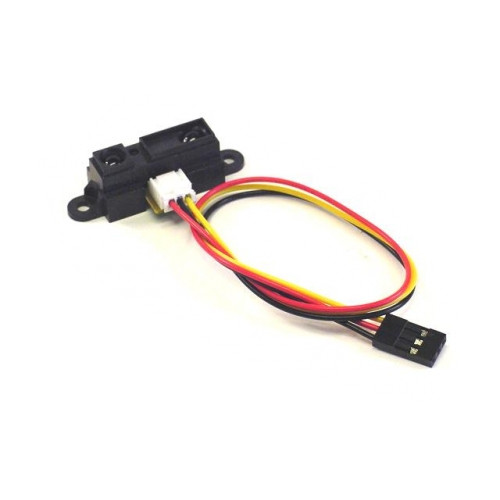
\includegraphics[width=0.9\linewidth]{sharp_ir}
            \end{center}
        \end{column}
    \end{columns}

\end{frame}

%%%%%%%%%%%%%%%%%%%%%%%%%%%%%%%%%%%%%%%%%%%%%%%%%%%%%%%%%%%%%%%%%%%%%%%%%%%%%%%%%%%%%%%%%%
\subsection{Structured Light}


\begin{frame}{Structured light (vision, 2D, 3D)}
    \only<1>{
        \begin{itemize}

            \item Eliminate the correspondence problem of stereo vision by projecting
                  structured light on the scene.
            \item Project slits of light or emits collimated light (\eg laser) by means
                  of a rotating mirror.
            \item Reflection sensed by camera.
            \item Range to an illuminated point can be determined from simple geometry.
        \end{itemize}
    }
    \only<2>{
        \begin{center}
            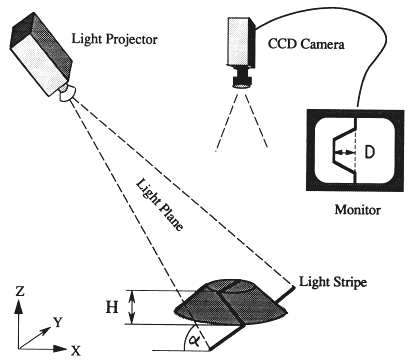
\includegraphics[width=0.6\linewidth]{2d-structured-light}

            \[
            H=D\cdot tan(\alpha)
            \]
        \end{center}
    }
    \only<3>{
        \begin{center}
            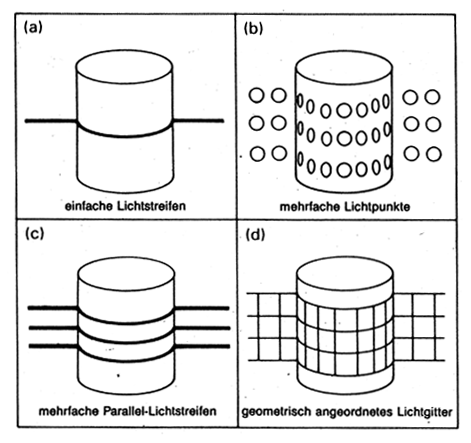
\includegraphics[width=0.7\linewidth]{structured-light-patterns}
        \end{center}
    }
\end{frame}

\begin{frame}{Structured light -- Principle}

    \only<1>{
        \begin{columns}
            \begin{column}{0.4\linewidth}

                One dimensional schematic of the principle.

                  From the figure, simple geometry shows that:

                  \[
                      x_{target}=\frac{b\cdot u}{f\cdot cot(\alpha) + u}
                    \]

                \[
                    z_{target}=\frac{b\cdot f}{f\cdot cot(\alpha) + u}
                    \]

            \end{column}
            \begin{column}{0.6\linewidth}
    \tikzset{
            camera/.pic = {
                \draw[fill,orange] (-2,-0.5) rectangle (-0.1,0.5);
                \draw[fill,orange] (-0.2,-0.1) rectangle (0,0.1);
                \node[label] at (-1,0) {laser};
            }
    }
    \begin{tikzpicture} 
        [>=latex,label/.style={align=center,font=\footnotesize}]

        \pgfmathsetmacro{\lensRadius}{3}
        \pgfmathsetmacro{\lensHeight}{1}
        \pgfmathsetmacro{\startAngle}{asin(\lensHeight/\lensRadius)}
        \pgfmathsetmacro{\incidenceAngle}{70}
    
        \coordinate (target) at (0,0);

        \coordinate (lens) at ($(target)+(\incidenceAngle:5)$);
        \coordinate (transmitter) at ($(target)+(180-\incidenceAngle:5)$);
        \coordinate (psd) at ($(lens) + (-1.5,0.5)$);
        \coordinate (psd2) at ($(psd) + (3,0.3)$);

        \coordinate (impact) at (intersection of target--lens and psd--psd2);

        \fill [red, opacity=0.5] (impact) circle (2pt);

        \path (transmitter) pic[scale=0.5,rotate=-\incidenceAngle]{camera};
        \draw[very thick,->] (transmitter) -- (target);

        \draw[dash pattern=on 2pt off 4pt on 6pt off 4pt] (transmitter) -- ($(lens) + (1.5,0)$);

        \draw[thick, dashed,->] (target) -- +(30:1);
        \draw[thick, dashed,->] (target) -- +(60:1);
        \draw[thick, dashed,->] (target) -- +(120:1);
        \draw[thick, dashed,->] (target) -- +(150:1);

        \draw[ultra thick] (target)++(1, 0) -- ++(-2,0) node[label,below,midway] {$(x_{target},z_{target})$};

        \draw[very thick, dashed,->] (target) -- (impact);

        \draw[<->] (2.8,0.5 |- lens) -- (2.8,1 |- psd) node[label, right,midway] {$f$};

        \draw[<->] (lens |- 3,4) -- (transmitter |- 3,4) node[label,below,midway] {baseline $b$};
        \draw ($(lens) + (0,0.5)$) -- ($(lens) + (0,-1.1)$);
        \draw (transmitter) -- ($(transmitter) + (0,-1.1)$);

        \draw (transmitter) + (0.5,0) arc [start angle=0, end angle=-\incidenceAngle, radius=0.5] node[midway,right] {$\alpha$};

        \draw[thick] (psd) rectangle (psd2);
        \foreach \a in {0.1,0.2,...,3}
            \draw ($(psd) + (\a,0)$) -- +(0,0.3);

        \draw[rotate=90,fill=blue!15, semitransparent]  ($(lens)+(0,\lensHeight)$)
        arc[start angle=180-\startAngle,delta angle=2*\startAngle,radius=\lensRadius]
          arc[start angle=-\startAngle,delta angle=2*\startAngle,radius=\lensRadius]
             -- cycle;

        \node[label,anchor=west] at ($(lens) + (0.5,-0.3)$) {Lens};
        \node[label,anchor=west] at ($(psd2) + (-0.5,0.3)$) {Camera};

        \coordinate (mirrorimpact) at ({$2*(lens) - (impact)$} |- impact);
        \draw[thin, dashed,shorten <=-0.4cm,shorten >=-0.5cm] (mirrorimpact) -- (lens);

        \draw (psd2 -| impact) -- +(0,0.3);
        \draw (psd2 -| mirrorimpact) -- +(0,0.3);
        \draw[<->] ({$(psd2) + (0,0.2)$} -| impact) -- ({$(psd2) + (0,0.2)$} -| mirrorimpact) node[label, above,midway] {$f\cdot cot\alpha + u$};

        \draw[thick,->] (lens) -- +(-1.5,0) node[label,left] {$x$};
        \draw[thick,->] (lens) -- +(0,-1.5) node[label,below] {$z$};
        \draw[thick,->] ($(psd)!0.5!(psd2)$) -- +(2,0) node[label,below] {$u$};
    \end{tikzpicture}

            \end{column}
        \end{columns}

    }

    \only<2-3>{
        Range resolution is defined as the \textbf{triangulation gain} $G_p$:

        \[
            \frac{\partial u}{\partial z} = G_p = \frac{b \cdot f}{z^2}
        \]

    \only<2>{
        \textbf{Baseline} length $b$

        \begin{itemize}

            \item the smaller $b$, the more compact the sensor can be.
            \item the larger $b$, the better the range resolution is.
        \end{itemize}

        \begin{exampleblock}{}
            However, for large $b$, the chance that an illuminated point is not
            visible to the receiver increases!
        \end{exampleblock}

    }
    \only<3>{

        \textbf{Focal length} $f$

        A larger focal length $f$ gives

        \begin{itemize}
            \item a smaller field of view
            \item an improved range resolution
            \item less lens distortion
            \item a larger sensor head
        \end{itemize}
    }
}
\end{frame}

%%%%%%%%%%%%%%%%%%%%%%%%%%%%%%%%%%%%%%%%%%%%%%%%%%%%%%%%%%%%%%%%%%%%%%%%%%%%%%%%%%%%%%%%%%
\subsection{Cameras}

\begin{frame}{Camera}

    \begin{columns}
        \begin{column}{0.5\linewidth}

            \textbf{Hardware}

            \begin{itemize}
                \item Two technologies: CCD or CMOS
                \item Monochrome or colour
                \item Resolution between 1 x 64 pixels and 4000 x 4000 pixels
                \item Small, low-power and cheap
                \item Prices anything between 40p and £3000

                    \begin{itemize}
                        \item Cameras have dropped significantly in price, and are the cheapest
                            high-tech sensor around
                    \end{itemize}

            \end{itemize}
        \end{column}
        \begin{column}{0.5\linewidth}
            \begin{center}
                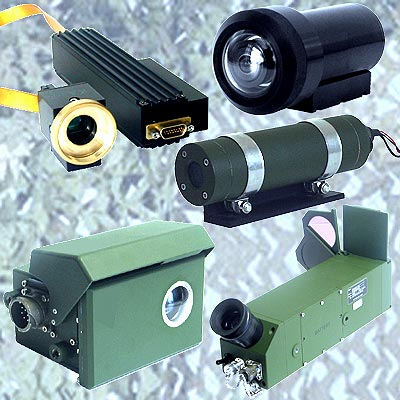
\includegraphics[width=0.7\linewidth]{camera1}

                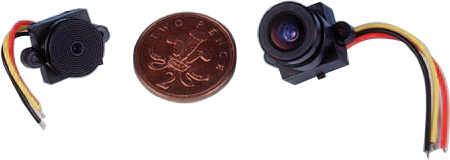
\includegraphics[width=0.8\linewidth]{camera2}

                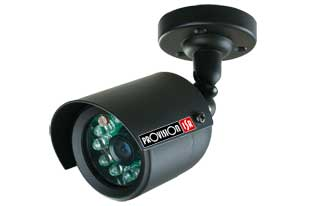
\includegraphics[width=0.6\linewidth]{camera3}
            \end{center}
        \end{column}
    \end{columns}
\end{frame}

\begin{frame}{Camera output}

    Most cameras provide digital output:

    \begin{itemize}

        \item
            USB1.0, USB1.1, USB2.0, USB3.0, Firewire (aka IEEE 1394 -- mostly replaced by USB3.0), Ethernet,
              or any hardware bus or proprietary bus (like on the Raspberry Pi).
    \end{itemize}

    Some --mostly older-- camera designs do not, and provide an analog (RGB
    or composite) signal instead.

    $\rightarrow$ a \textbf{frame grabber} is needed to digitise the signal.
    Matrox is the leading manufacturer of frame grabbers.

    \begin{center}
        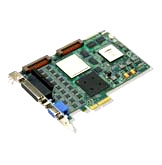
\includegraphics[width=0.25\linewidth]{matrox-framegrabber1}
        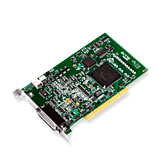
\includegraphics[width=0.25\linewidth]{matrox-framegrabber2}
    \end{center}

\end{frame}

\begin{frame}{Camera parameters}

    \textbf{Shutter speed}

    Rate at which an image is refreshed, \eg 25ms, 1/400 s.

    \textbf{Iris position} (aka \textbf{aperture})

    Size of the lens opening, mechanically operated. Allows more or less light
    in.

    \textbf{Camera gain}

    Amplification of the camera signal. \emph{Noise is amplified as well.}

    \textbf{White balance} (aka color temperature)

    Mixture of blue, red and green components that define white. Often needed
    to cancel out influences of illumination.

\end{frame}

\begin{frame}{CCD technology}

    \only<1>{
        \textbf{Charge-coupled device} (\emph{CCD})
    \begin{columns}
        \begin{column}{0.55\linewidth}

        \begin{itemize}

            \item Each pixel has a photodiode and a capacitor, the capacitor is charged
                  or discharged as photons hit the light-sensitive silicon.
            \item The charge in the capacitor is proportional to the light intensity.
            \item The charge is read out at the corner of the chip's surface.
            \item Charge is transferred over the chip' surface to that corner, like a
                  ``bucket brigade''.
        \end{itemize}
            
        \end{column}
        \begin{column}{0.45\linewidth}
            \begin{center}
                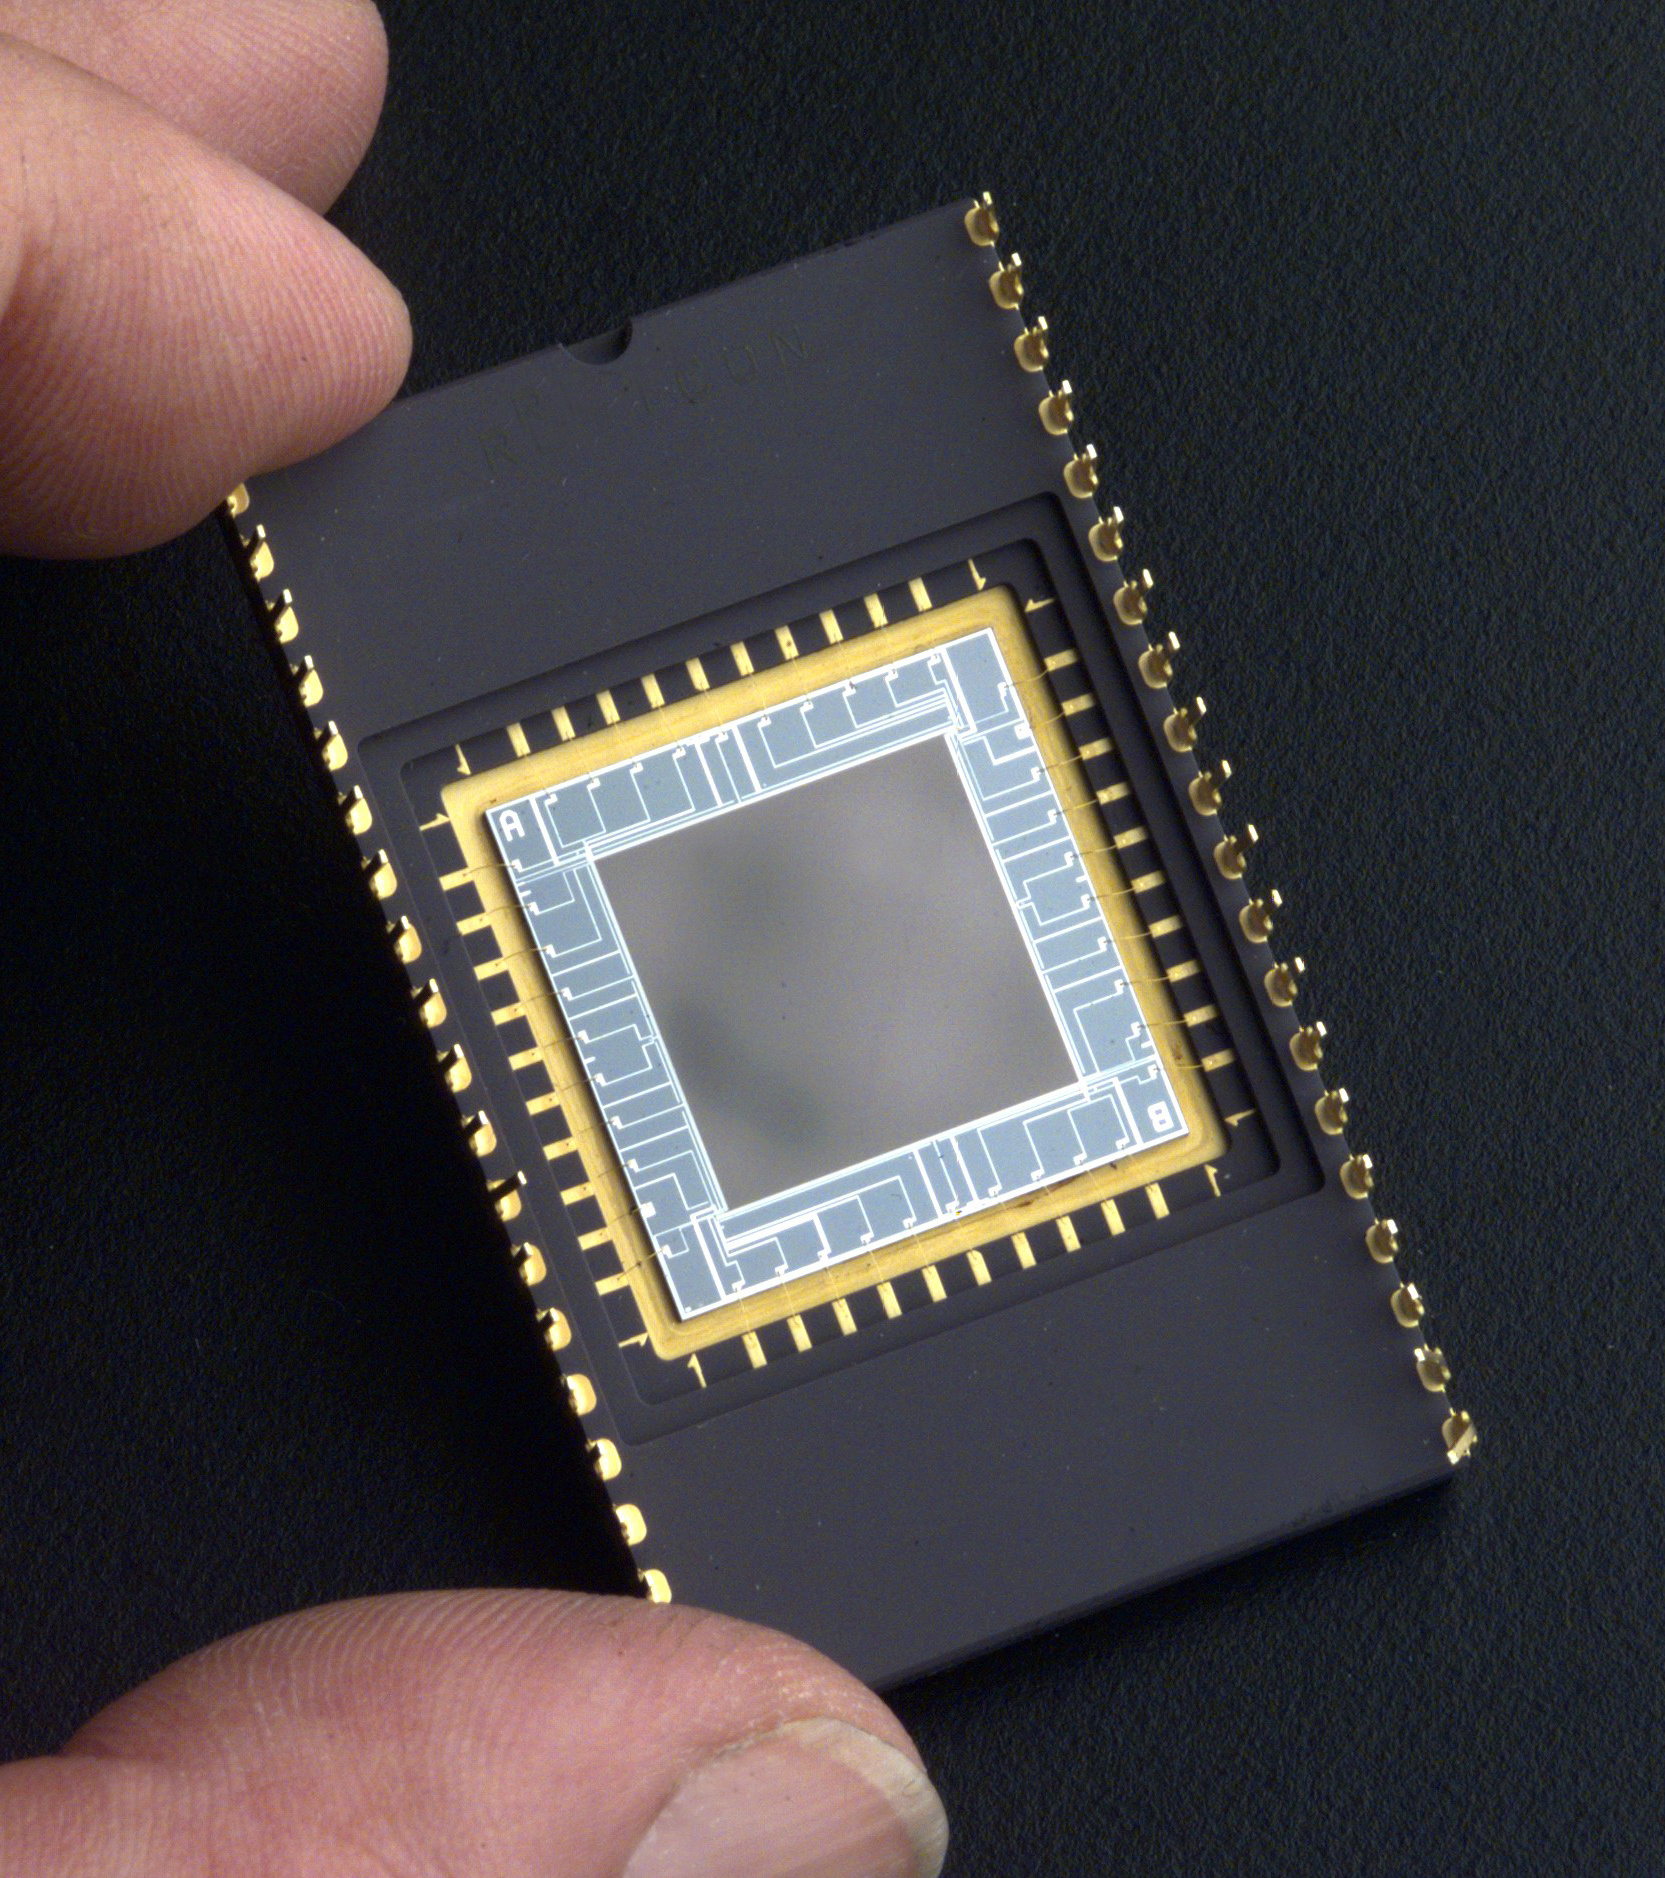
\includegraphics[width=0.8\linewidth]{ccd}

                \source{https://en.wikipedia.org/wiki/File:Delta-Doped_Charged_Coupled_Devices_(CCD)_for_Ultra-Violet_and_Visible_Detection.jpg}{Wikipedia}
            \end{center}

            \href{http://www.optique-ingenieur.org/en/courses/OPI_ang_M05_C06/co/Contenu_04.html}{More details on CCD sensors}
        \end{column}
    \end{columns}
    }
    \only<2>{

        Some sort of shutter is needed to prevent smear in the camera image.

        \begin{itemize}

            \item \emph{Mechanical shutter}: expensive and high power consumption.
            \item \emph{Frame transfer CCD}: one half of the chip's surface is opaque, charge
                  is transferred there and then read out.
              \item \emph{Interline architecture}: every other line is opaque, faster shutter
                  speeds possible. Less sensitive to light.
        \end{itemize}


    }
    \only<3>{
        Available sensors can function from far infrared (100$\mu$m) to X-rays
        (1nm).

        Common sensors in the range 400nm -- 1000nm $\Rightarrow$ Human visual
        spectrum from 380nm to 780nm, so \emph{less sensitive to blue light}
        and \emph{oversensitive to red and infrared}.

    }
    \only<4>{

        \textbf{CCD -- advantages}

        \begin{itemize}
            \item high quality, relatively low noise images
            \item high quantum efficiency

                \begin{itemize}

                    \item
                        70 to 80\% of photons are converted into a charge, ideal for low light
                        conditions.
                \end{itemize}

            \item \emph{integrating function} of pixels.
                \begin{itemize}
                    \item can be used to measure for prolonged times in very dim settings.
                \end{itemize}
        \end{itemize}
    }

    \only<5>{

        \textbf{CCD -- disadvantages}

        \begin{itemize}
            \item integrating light measurement
                \begin{itemize}
                    \item in bright light, capacitors can \textbf{saturate}
                    \item saturation leads to charge leaks from one pixel to
                        the other: causes \textbf{blooming} the image
                \end{itemize}
            \item large silicon size due to circuitry to read out pixels
            \item interfacing between CCD and CMOS technology is not straight-forward
                \begin{itemize}
                    \item hinders cheap hardware
                \end{itemize}
            \item complex clocking issues on chip
            \item large dissipation
        \end{itemize}
    }
\end{frame}

\begin{frame}{CMOS technology}

    \only<1>{
        \textbf{Complementary Metal Oxide Semiconductor} (\emph{CMOS})

        \begin{columns}
            \begin{column}{0.5\linewidth}
        \begin{itemize}

            \item Photodiode with circuitry that reads out light intensity.
            \item \textbf{No} integrating measurement, but a \textbf{proportional}
                  measurement instead.
            \item Pixel values are read out much like in RAM memory.
        \end{itemize}
                
            \end{column}
            \begin{column}{0.5\linewidth}
                \begin{center}
                    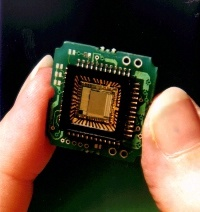
\includegraphics[width=0.8\linewidth]{cmos}
                \end{center}
            \end{column}
        \end{columns}

    }
    \only<2>{
        \textbf{CMOS -- advantages}

        \begin{itemize}
            \item CMOS technology is mature and simple
                \begin{itemize}
                    \item Production costs are a fraction of that of CCD.
                \end{itemize}
            \item No complex clocking in chip.
            \item Low power consumption.
            \item Proportional measurement
                \begin{itemize}
                    \item $\rightarrow$ no saturation of pixels.
                \end{itemize}
            \item Smaller silicon size.
            \item Random access to pixels (just like RAM).
            \item Easy interfacing to CMOS technology.
                \begin{itemize}
                    \item CMOS circuitry, \eg for bus, can be integrated on the same silicon
                        area.
                \end{itemize}
        \end{itemize}
    }
    \only<3>{
        \textbf{CMOS -- disadvantages}

        \begin{itemize}
            \item Each photodiode has CMOS circuitry which takes up silicon
                real estate, but is not sensitive to incoming light
                \begin{itemize}
                    \item CMOS camera is less sensitive than CCD.
                \end{itemize}
            \item CMOS has a larger pixel mismatch and is typically more noisy than
                CCD.
                \begin{itemize}
                    \item This has improved considerably over the years, see CMOS in high-end
                        \#\# digital cameras.
                \end{itemize}
        \end{itemize}

    }

\end{frame}

\imageframe{ccd-vs-cmos}

\begin{frame}{Colour cameras}
    \only<1>{
        With one CCD or CMOS sensor, a filter is placed in front of the sensor
        surface.

        \begin{itemize}

            \item Resolution, relative to monochrome camera, is reduced by 75\%
            \item Bayer (GRGB) or RGBE (E = Emerald) filter
        \end{itemize}

        \begin{columns}
            \begin{column}{0.5\linewidth}
                \begin{center}
                    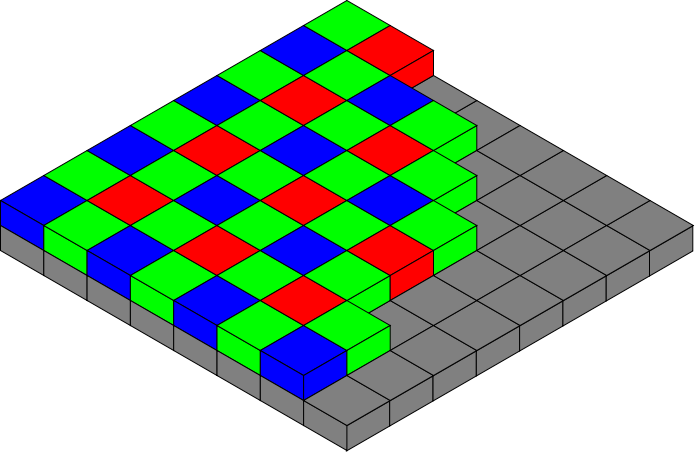
\includegraphics[width=0.8\linewidth]{bayer}

                    Bayer filter
                \end{center}

            \end{column}
            \begin{column}{0.5\linewidth}
                \begin{center}
                    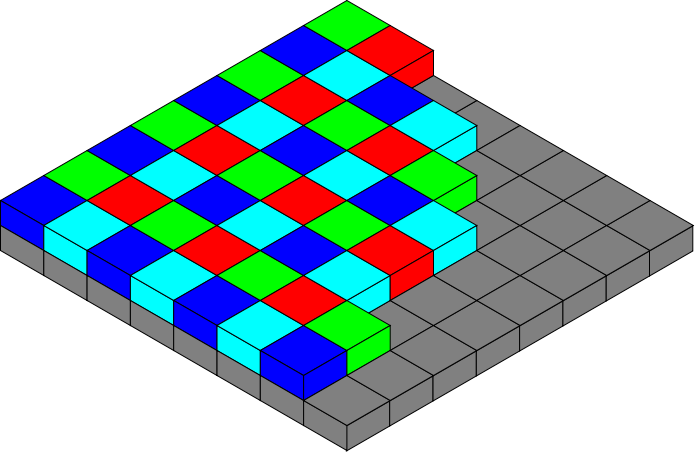
\includegraphics[width=0.8\linewidth]{rgbe}

                RGBE filter
                \end{center}

            \end{column}
        \end{columns}

    }
    \only<2>{

        Three sensor cameras.

        \begin{itemize}
            \item In expensive and professional colour cameras, the images is optically
                  split in three.
            \item Each copy is sent to a separate sensor, each sensor has a R, G, or B
                  filter.
        \end{itemize}

        $\Rightarrow$ No resolution loss due to Bayer or RGBE filter

        $\Rightarrow$ No problem of misalignment of filter

    }
\end{frame}

\begin{frame}{Omnidirectional camera}

              Most robots need 360° vision, this can be provided by a
              \textbf{omnidirectional camera}.

    \begin{center}
        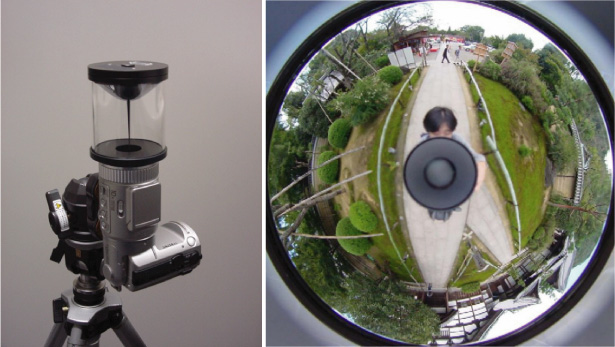
\includegraphics[width=0.8\linewidth]{omni}
    \end{center}
\end{frame}

\begin{frame}{Image processing and computer vision}

    \begin{itemize}

        \item
              See Phil Culverhouse's lectures.
        \item
              Take an MSc Robotics next year.
    \end{itemize}

\end{frame}

%%%%%%%%%%%%%%%%%%%%%%%%%%%%%%%%%%%%%%%%%%%%%%%%%%%%%%%%%%%%%%%%%%%%%%%%%%%%%%%%%%%%%%%%%%
\subsection{RGB-D cameras}

\begin{frame}{RGB-D cameras: many technologies}
    \begin{itemize}
        \item Stereo-vision
        \item Structured light
        \item Speckle decorrelation
        \item Time-of-Flight
        \item (...several other like coded-aperture)
    \end{itemize}
\end{frame}

\imageframe{depthmap}

\imageframe{stereo_head}

\begin{frame}{Stereovision}

    \only<1>{
        \begin{itemize}

            \item A camera typically forms a 2D mapping of a 3D environment.
            \item Reconstructing depth from a 2D image is in most cases impossible.
            \item A solution to this is using a \textbf{stereo camera} which can
                  calculate the depth (\ie $z$ axis) of pixels.
            \item Using two slightly different views from the same scene and a precise
                  knowledge of camera parameters.
        \end{itemize}

        \begin{center}
            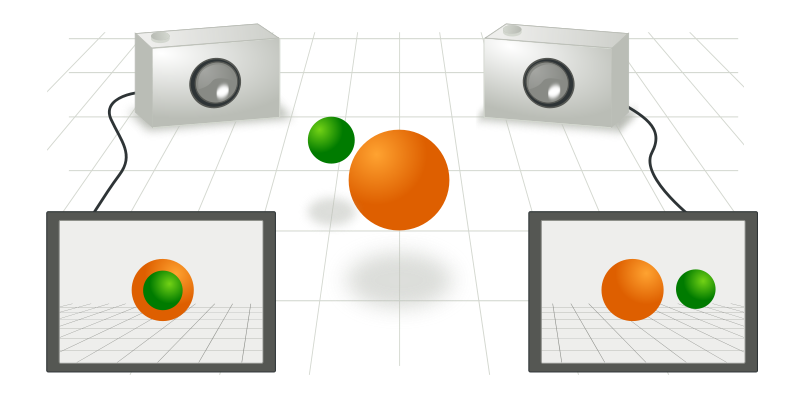
\includegraphics[width=0.6\linewidth]{stereo_principle}

            \source{}{Wikipedia}
        \end{center}
    }

    \only<2>{

        \begin{multicols}{2}

            \begin{center}
                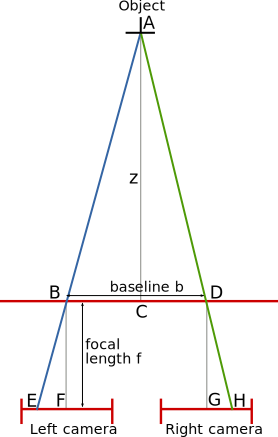
\includegraphics[height=0.8\paperheight]{stereo}
            \end{center}

            \begin{align}
                d & = EF + GH                                        \\
                  & = BF (\frac{EF}{BF} + \frac{GH}{BF})             \\
                  & = BF (\frac{EF}{BF} + \frac{GH}{DG})             \\
                  & = BF (\frac{BC + CD}{AC})                        \\
                  & = BF \frac{BD}{AC} = \frac{k}{z}  \text{, where}
            \end{align}

            $k = BD \times BF = b \times f$\\
            $z = AC$

            $d$ is the \textbf{disparity}
        \end{multicols}

    }
    \only<3>{

        \textbf{Disparity map}

        Pixel disparity: for each {\bf pixel patch} on the left, by how many pixel the
        same patch is {\bf shifted} on the right?

        \begin{center}
            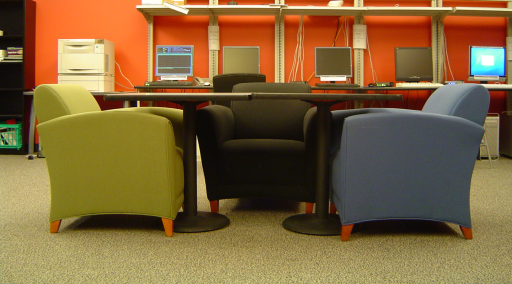
\includegraphics[width=0.45\linewidth]{scene_left}
            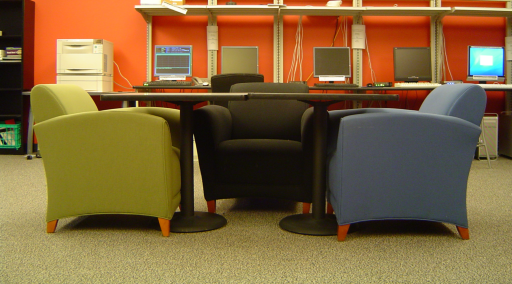
\includegraphics[width=0.45\linewidth]{scene_right}

            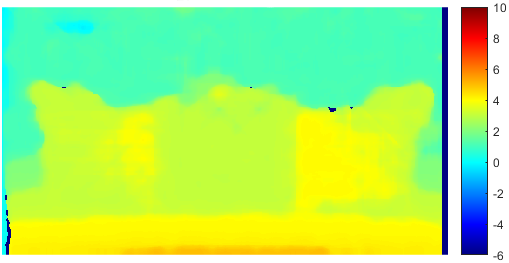
\includegraphics[width=0.45\linewidth]{disparity}
        \end{center}
    }

    \only<4>{

        \textbf{Advantages}

        \begin{itemize}
            \item Simple technology
            \item Works great outdoors
        \end{itemize}

        \textbf{Disadvantages}

        \begin{itemize}
            \item Two calibrated cameras needed
            \item Multiple computationally intensive steps
            \item Depends on illumination and scene texture
            \item Requires texture $\Rightarrow$ active stereovision
        \end{itemize}


    }
\end{frame}

\begin{frame}{Swissranger 3D camera}

    MESA SR3000

    \begin{itemize}

        \item
              Uses TOF measured as phase difference of IR light.
        \item
              CCD camera at 176 x 144 resolution.
        \item
              Frame rate, 29fps at 0.3m to 12fps at 3m.
        \item
              Accuracy: 3mm (best case).
        \item
              \$7500 (in 2008)
    \end{itemize}

\end{frame}

\begin{frame}{Microsoft Kinect}

    \textbf{Kinect 360} (also known as version 1). Released in 2010.

    \textbf{Kinect One} (also known as version 2). Released in 2014.

\end{frame}

\begin{frame}{Kinect 360 - Primesense 3D camera}

    Infrared laser light pattern projected onto scene and filmed with CMOS
    camera.

    \begin{itemize}

        \item
              Class 1 laser device: safe for eyes.
        \item
              1cm depth resolution, 3mm height and width.
        \item
              320x240 16-bit depth @ 30 frames/sec, 640x480 32-bit colour@ 30
              frames/sec, 16-bit audio @ 16 kHz
        \item
              Stronger light than Swissranger 3D cam: laser dots vs LED light.
    \end{itemize}

\end{frame}

\begin{frame}{Kinect 360 - Primesense 3D camera}

    The hardware is only one aspect of the sensor.

    The software is equally important.

    \begin{itemize}

        \item
              Matching a cloud of points in 3D space to 2 body models is a very hard
              problem in artificial intelligence.
        \item
              Machine learning used to let the software learn mapping between 3D
              points and body models (see
              \href{http://www.theinstitute.ieee.org/portal/site/tionline/menuitem.130a3558587d56e8fb2275875bac26c8/index.jsp?\&pName=institute_level1_article\&TheCat=2201\&article=tionline/legacy/inst2011/jan11/featuretech.xml\&}{IEEE
              article})
    \end{itemize}

\end{frame}

\begin{frame}{Kinect 360 - Primesense 3D camera}

    Principles

    \begin{itemize}

        \item
              Dot pattern (speckles) is projected in near IR light.
        \item
              CMOS IR camera records image.
        \item
              Pattern is known by sensor. Calibration is done at time of
              manufacturing: a set of calibration images is stored in the device.
        \item
              Each dot pattern encodes a coordinate
    \end{itemize}

    From
    \href{http://worldwide.espacenet.com/publicationDetails/originalDocument?FT=D\&date=20100909\&DB=EPODOC\&locale=en_EP\&CC=US\&NR=2010225746A1\&KC=A1}{US
    Patent}

    More at
    \href{http://campar.in.tum.de/twiki/pub/Chair/TeachingSs11Kinect/2011-DSensors_LabCourse_Kinect.pdf}{TUM}

\end{frame}

\begin{frame}{Kinect skeleton tracking}

    \begin{itemize}

        \item
              Reading depth image is only one part what the Kinect does.
        \item
              It also infers skeleton (positions of torse, head, arms and legs) from
              depth image.
        \item
              Based on machine learning
              (\href{http://research.microsoft.com/pubs/145347/BodyPartRecognition.pdf}{Shotton
              et al., 2011})
    \end{itemize}

\end{frame}

\begin{frame}{Machine learning}

    100,000 images of people in front of RGBD sensor, together with ``ground
    truth'' from a motion capture system.

    \begin{itemize}

        \item
              Different body types, different clothes.
    \end{itemize}

    Using machine learning (\emph{randomised decision forest} algorithm) to
    find body parts

    \begin{itemize}

        \item
              A farm of computers required a day to arrive at a solution to separate
              body parts from background images.
    \end{itemize}

    Microsoft SDK allows tracking of 2 skeleton for Kinect 360 and 5 for
    Kinect One.

\end{frame}

\begin{frame}{The Kinect One}

    The same, but better!

    \begin{itemize}

        \item
              Faster full HD video stream
        \item
              Better microphones
        \item
              Higher depth fidelity
        \item
              Wider angle camera (70x60 degrees vs K1 57x43)
        \item
              Improved skeleton model (prediction)
        \item
              More skeleton points (26)/more people tracked (6 full)
        \item
              New development SDK
        \item
              More expensive, not as much support as yet
        \item
              CANNOT use Xbox version with PC like with v1!
    \end{itemize}

\end{frame}

\begin{frame}{360 vs One Technology}

    \begin{itemize}

        \item
              Kinect 360 project speckle pattern into environment, uses
              triangulation (structured light) from near-IR
    \end{itemize}

    (WikiMedia)

\end{frame}

\begin{frame}{360 vs One Technology}

    Kinect One uses Time-of-Flight (indirectly measured through phase shift
    measurements).

    Take 2 measurements -- eliminate ambiguity if light is absorbed

    Ambient light rejection

    \begin{itemize}

        \item
              Allows outdoor operation!
    \end{itemize}

    Excellent explanation
    \href{http://www.gamasutra.com/blogs/DanielLau/20131127/205820/The_Science_Behind_Kinects_or_Kinect_10_versus_20.php}{here}

\end{frame}

\begin{frame}{How do we use it?}

    \only<1>{
        2 main options:

        \begin{itemize}

            \item
                  1. Microsoft SDK
            \item
                  2. OpenNI
        \end{itemize}

        Microsoft SDK needs specific versions of Visual Studio

        Microsoft SDK is best complemented with the Developer Tools (which has
        lots of great example applications)

    }
    \only<2>{
        Lots of cables -- plug the Kinect into the power adapter, then the USB
        to your computer

        \begin{itemize}

            \item
                  Make sure the power is on before you plug it in to a PC, or it will
                  see it only as a microphone
        \end{itemize}

    }
    \only<3>{
        The Microsoft SDK can be programmed with C\#.Net, VB.Net or VC++

        \begin{itemize}

            \item
                  We recommend C\#, but C++ is possible as well
        \end{itemize}

        Or if you want to try, there are other options as well

        \begin{itemize}

            \item
                  \href{https://processing.org/}{Processing} is a language for
                  non-programmers with excellent support for Kinect (see
                  \href{http://shiffman.net/p5/kinect/}{here})
        \end{itemize}
    }
\end{frame}

\begin{frame}{Programming principles}

    \begin{itemize}

        \item
              SDK provides interface to find and use sensor in just a few lines
        \item
              Events fire when a new RGB frame or depth frame are ready for use, or
              when audio source changes angle or energy
        \item
              We put a handler on these events to pick up the images
        \item
              We can then read out raw data values, convert images, or use the
              processed data about skeletons/faces
        \item
              Continuous audio processing must be done manually in its own thread
    \end{itemize}

\end{frame}

%%%%%%%%%%%%%%%%%%%%%%%%%%%%%%%%%%%%%%%%%%%%%%%%%%%%%%%%%%%%%%%%%%%%%%%%%%%%%%%%%%%%%%%%%%%%%%%%%
%%%%%%%%%%%%%%%%%%%%%%%%%%%%%%%%%%%%%%%%%%%%%%%%%%%%%%%%%%%%%%%%%%%%%%%%%%%%%%%%%%%%%%%%%%%%%%%%%
\section{Applications in robotics}

\begin{frame}{In robotics applications}

    \textbf{Tele-operation:}

    \begin{itemize}

        \item
              Plymouth: \url{https://www.youtube.com/watch?v=wf4waMhPHmc}
        \item
              Plymouth Baxter: \url{https://www.youtube.com/watch?v=XKRI0hcInqE}
        \item
              NASA: \url{https://www.youtube.com/watch?v=pqNC72fgetc}
        \item
              Full body: \url{https://www.youtube.com/watch?v=7vq-1TiXi3g}
        \item
              2 arms: \url{https://www.youtube.com/watch?v=kECNyr7v0kM}
    \end{itemize}

    Autonomous navigation: \url{https://www.youtube.com/watch?v=eWmVrfjDCyw}

    Cutting bananas?:
    \url{https://www.youtube.com/watch?v=TmTW61MLm68\#t=356}

\end{frame}


\begin{frame}{}
    \begin{center}
        \Large
        That's all, folks!\\[2em]
        \normalsize
        Questions:\\
        Portland Square A216 or \url{severin.lemaignan@plymouth.ac.uk} \\[1em]

        Slides:\\ \href{https://github.com/severin-lemaignan/module-mobile-and-humanoid-robots}{\small github.com/severin-lemaignan/module-mobile-and-humanoid-robots}

    \end{center}
\end{frame}



\end{document}
